%%
% Please see https://bitbucket.org/rivanvx/beamer/wiki/Home for obtaining beamer.
%%

% La clase beamer requiere necesariamente la compilación mediante pdfLaTeX

\documentclass[9pt]{beamer}

% Incluir los paquetes
% Packages
\usepackage[utf8]{inputenc}
\usepackage{graphicx}
\usepackage{enumerate}
\usepackage{hyperref}
\usepackage[spanish]{babel} 
\usepackage{listings}
\usepackage{tikz}
\usepackage{lettrine}
\usepackage[T1]{fontenc}
\usepackage{palatino} 
\usepackage{type1ec}
\usepackage{amsmath}
\usepackage{lmodern} 
\usepackage{type1cm}
\usepackage{cite}
\usepackage{amsthm}
\usepackage{lscape} 
\usepackage{upgreek} % para poner letras griegas sin cursiva
\usepackage{cancel} % para tachar
\usepackage{mathdots} % para el comando \iddots
\usepackage{mathrsfs} % para formato de letra
\usepackage{stackrel} % para el comando \stackbin
\usepackage{dsfont}
\usepackage{verbatim} %Para usar verbatiminput para el codigo fuente
\usepackage{color}

\usepackage{pdfpages}
\usepackage{multirow}	% Para poder unir filas en las tablas

\usepackage{colortbl}	% Para colorear tablas
\usepackage{pifont}
\usepackage{fancyhdr} %gestión de cabeceras y pies de página

%\usepackage{endnotes}	%notas al final del documento
\usepackage{blindtext}
\usepackage{tabularx}

%\usepackage[toc,style=altlistgroup,hyperfirst=false]{glossaries}

\usepackage{graphicx}
\usepackage{booktabs}
%\usepackage{multicols}
\usepackage{listings}


% Definiciones

%Teorema -> thm
\theoremstyle{plain}
		\newtheorem{thm}{Teorema}
		
% Definicion -> defn
\theoremstyle{definition}
	\newtheorem{defn}{Descripción}
	\newtheorem{exmp}{Ejemplo}

% Nota -> rem
\theoremstyle{remark}
	\newtheorem{rem}{Nota}
	
\setbeamercolor{postit}{fg=black,bg=yellow}


\mode<presentation>{\usetheme{Madrid}
} %Antibes-crane

\setbeamercovered{transparent=20}


\begin{document}
	% Portada y tabla de contenido
	% Configuración del titlepage
	\title{Electrocardiógrafo}
	\author[José, Paula, Pablo, Cristina, Celia, Ana ]{
			José Antonio Córdoba Gómez \\
			Paula de la Hoz Garrido \\
			Juan Pablo Sáez \\
			Cristina Garrido López \\
			Celia Pedregosa Moreno \\	
			Ana Isabel Guerrero Tejera
			}
	\institute[ETSIIT]{Escuela Técnica Superior de Ingeniería Informática y Telecomunicaciones}
	\date{\today}
	
\frame{\titlepage}

	\begin{frame}{Tabla de Contenidos}
		\tableofcontents
	\end{frame}
	
	
	% Contenido en sí
	% Una archivo por transparencia ayuda a la compilación
	%\logo{
\includegraphics[height=0.8cm]{images/ugr}}%\vspace{200pt}}
	\section[Introducción]{Introducción}
\begin{frame}[plain]
	\frametitle{Descripción del problema}
	
	
	\begin{defn}
	Sea un vector \textit{v} de números de tamaño \textit{n}, todos distintos, de forma que existe un índice \textit{p} (que no es ni el primero ni el último) tal que a la \textbf{izquierda de 	\textit{p} } los números están ordenados de forma \textbf{creciente} y a la \textbf{derecha} de \textit{p} están ordenados de forma \textbf{decreciente}; es decir \\
	
		\begin{equation}
			 \forall i,j \leq p, i < j \Rightarrow v[i] < v[j]  \hspace*{0.18in} \textbf{y} \hspace*{0.18in}  \forall i,j \geq p, i < j \Rightarrow v[i] > v[j] 
		\end{equation}
		\vspace*{0.05in}
		
	\end{defn}
\end{frame}
	
	
%	\begin{block}{Algoritmos que vamos a estudiar}
%			\begin{itemize}[<+-| alert@+>]
%				\item Burbuja
%				\item Inserción
%				\item Selección
%				\item Mergesort
%				\item Quicksort
%				\item Heapsort
%				\item Floyd
%				\item Hanoi
%			\end{itemize}	
%		\end{block}


%\input{Images/Explicacion}
	
	
%	%Contenido
%		\begin{block}{Título de bloque}
%			\begin{itemize}[<+-| alert@+>]
%				\item Gerardo es tonto \pause
%				\item Gerardo es más tonto aún \pause
%				\item Gerardo es gilipollas
%			\end{itemize}	
%		\end{block}
%		\pause
%
%		\begin{alertblock}{Importante}
%			Quien no tenga hoy hecho  el constructor por defecto de la clase fecha, ¡No aprueba conmigo!
%		\end{alertblock}
%		
%		\pause
%		
%		\begin{exampleblock}{Ejemplo}
%			De alguna manera...
%		\end{exampleblock}
%		
%		\pause


	

	\section[Algoritmo Bruto]{Algoritmo Bruto}
\begin{frame}[plain]
	\frametitle{Resolución}
		\begin{exampleblock}{Estrategia de resolución}
			Recorremos la estructura de datos desde el inicio y buscamos el \textbf{primer y único} elemento máximo que encontremos.
		\end{exampleblock}
		
\end{frame}		




\begin{frame}[plain]
	\frametitle{Breve explicación}
		\begin{figure}[htb]
		\begin{center}
		\begin{picture}(160,0)
		\put(-86,-70){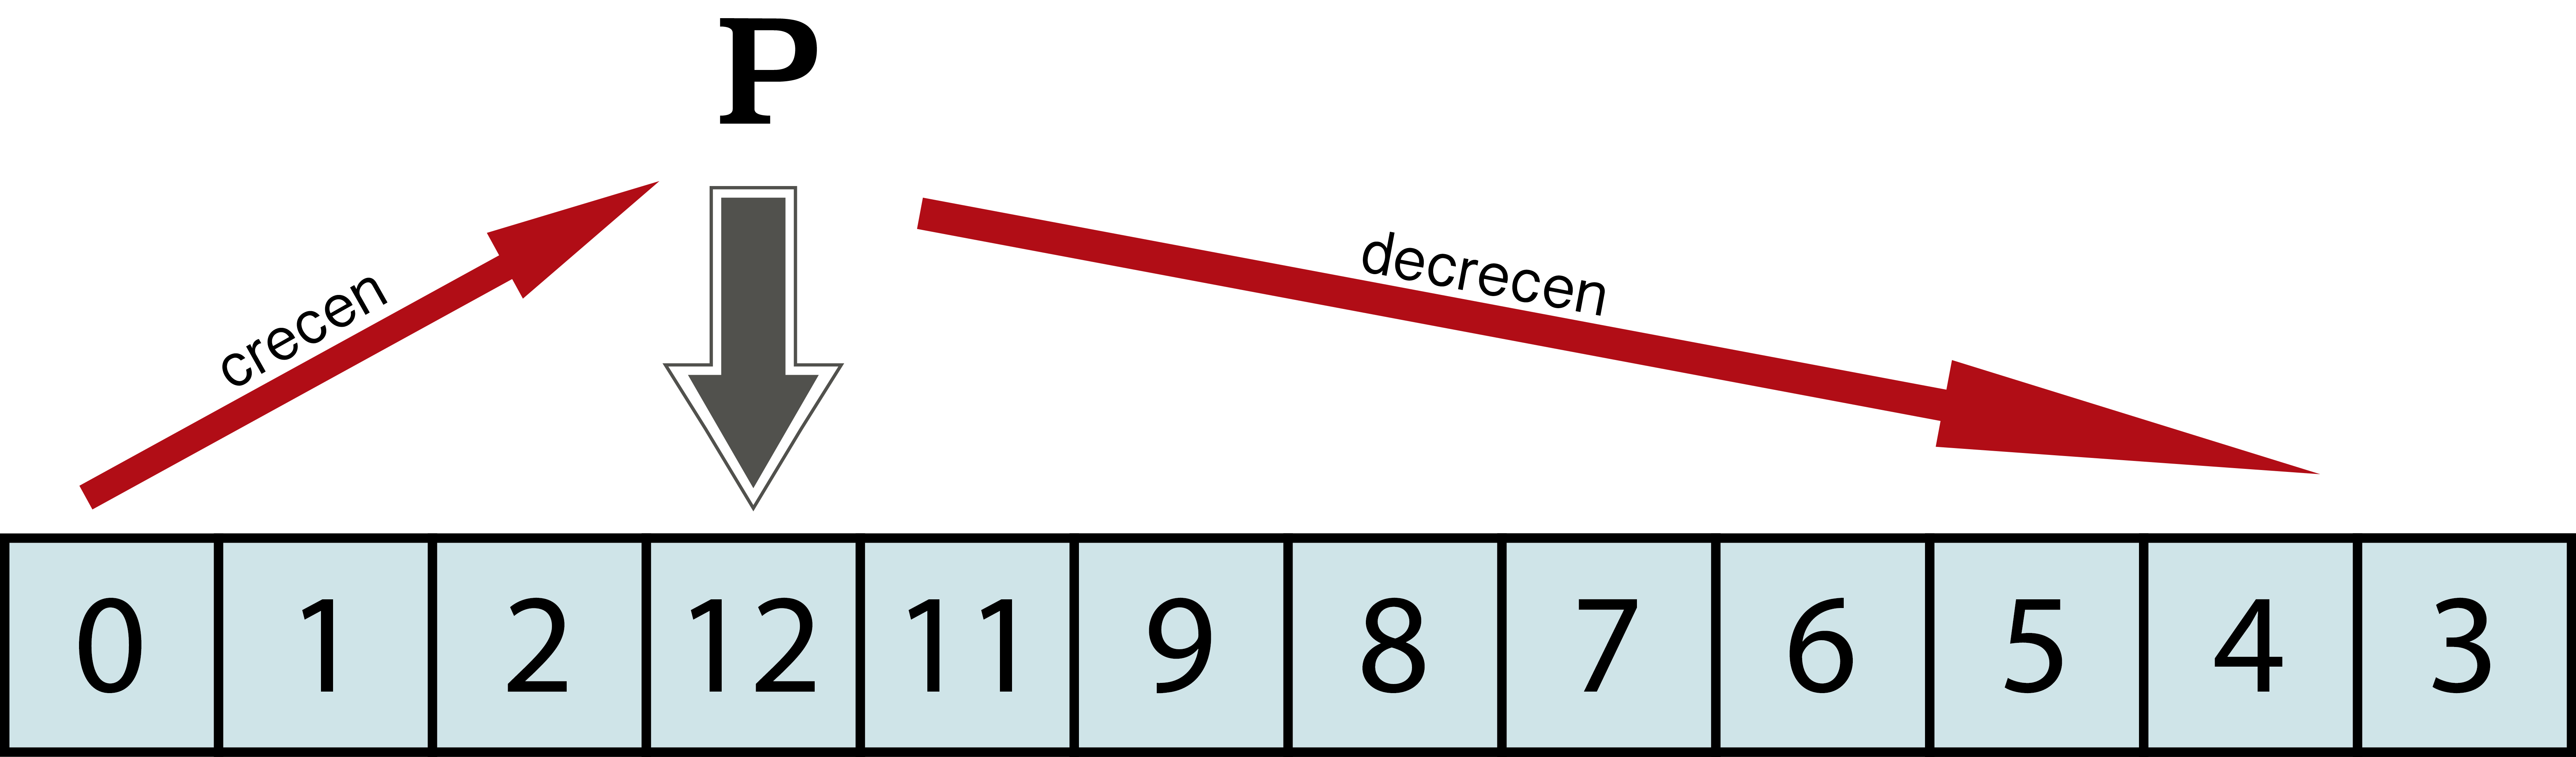
\includegraphics[width=11.5cm,height=4.0cm]{Images/Explicacion}}
		\end{picture}
		\end{center}
		\end{figure}
		
\end{frame}	




\begin{frame}[fragile]
	\frametitle{Algoritmo Bruto - Implementación}
	\lstset{language=C++,
                basicstyle=\ttfamily,
                tabsize=3, 
				showstringspaces=false,
				extendedchars=true,
                keywordstyle=\color{blue}\ttfamily,
                stringstyle=\color{red}\ttfamily,
                commentstyle=\color{yellow}\ttfamily,
                morecomment=[l][\color{magenta}]{\#}
     }
			\vspace*{-0.1in}
\begin{lstlisting}
int unimodalBruto(vector<int> v, int size){
bool found = false;
int pos = 0;

for(int i=0; i< size-1 && !found; i++)
   if(v[i]>v[i+1]){
      pos = i;
      found = true;
   }
    
if(found == false)
	pos = size-1;
return pos;
}

			\end{lstlisting}
	
	
			
\end{frame}	


\begin{frame}[plain]
	\frametitle{Breve explicación}
		\begin{figure}[htb]
		\begin{center}
		\begin{picture}(160,0)
		\put(-50,-110){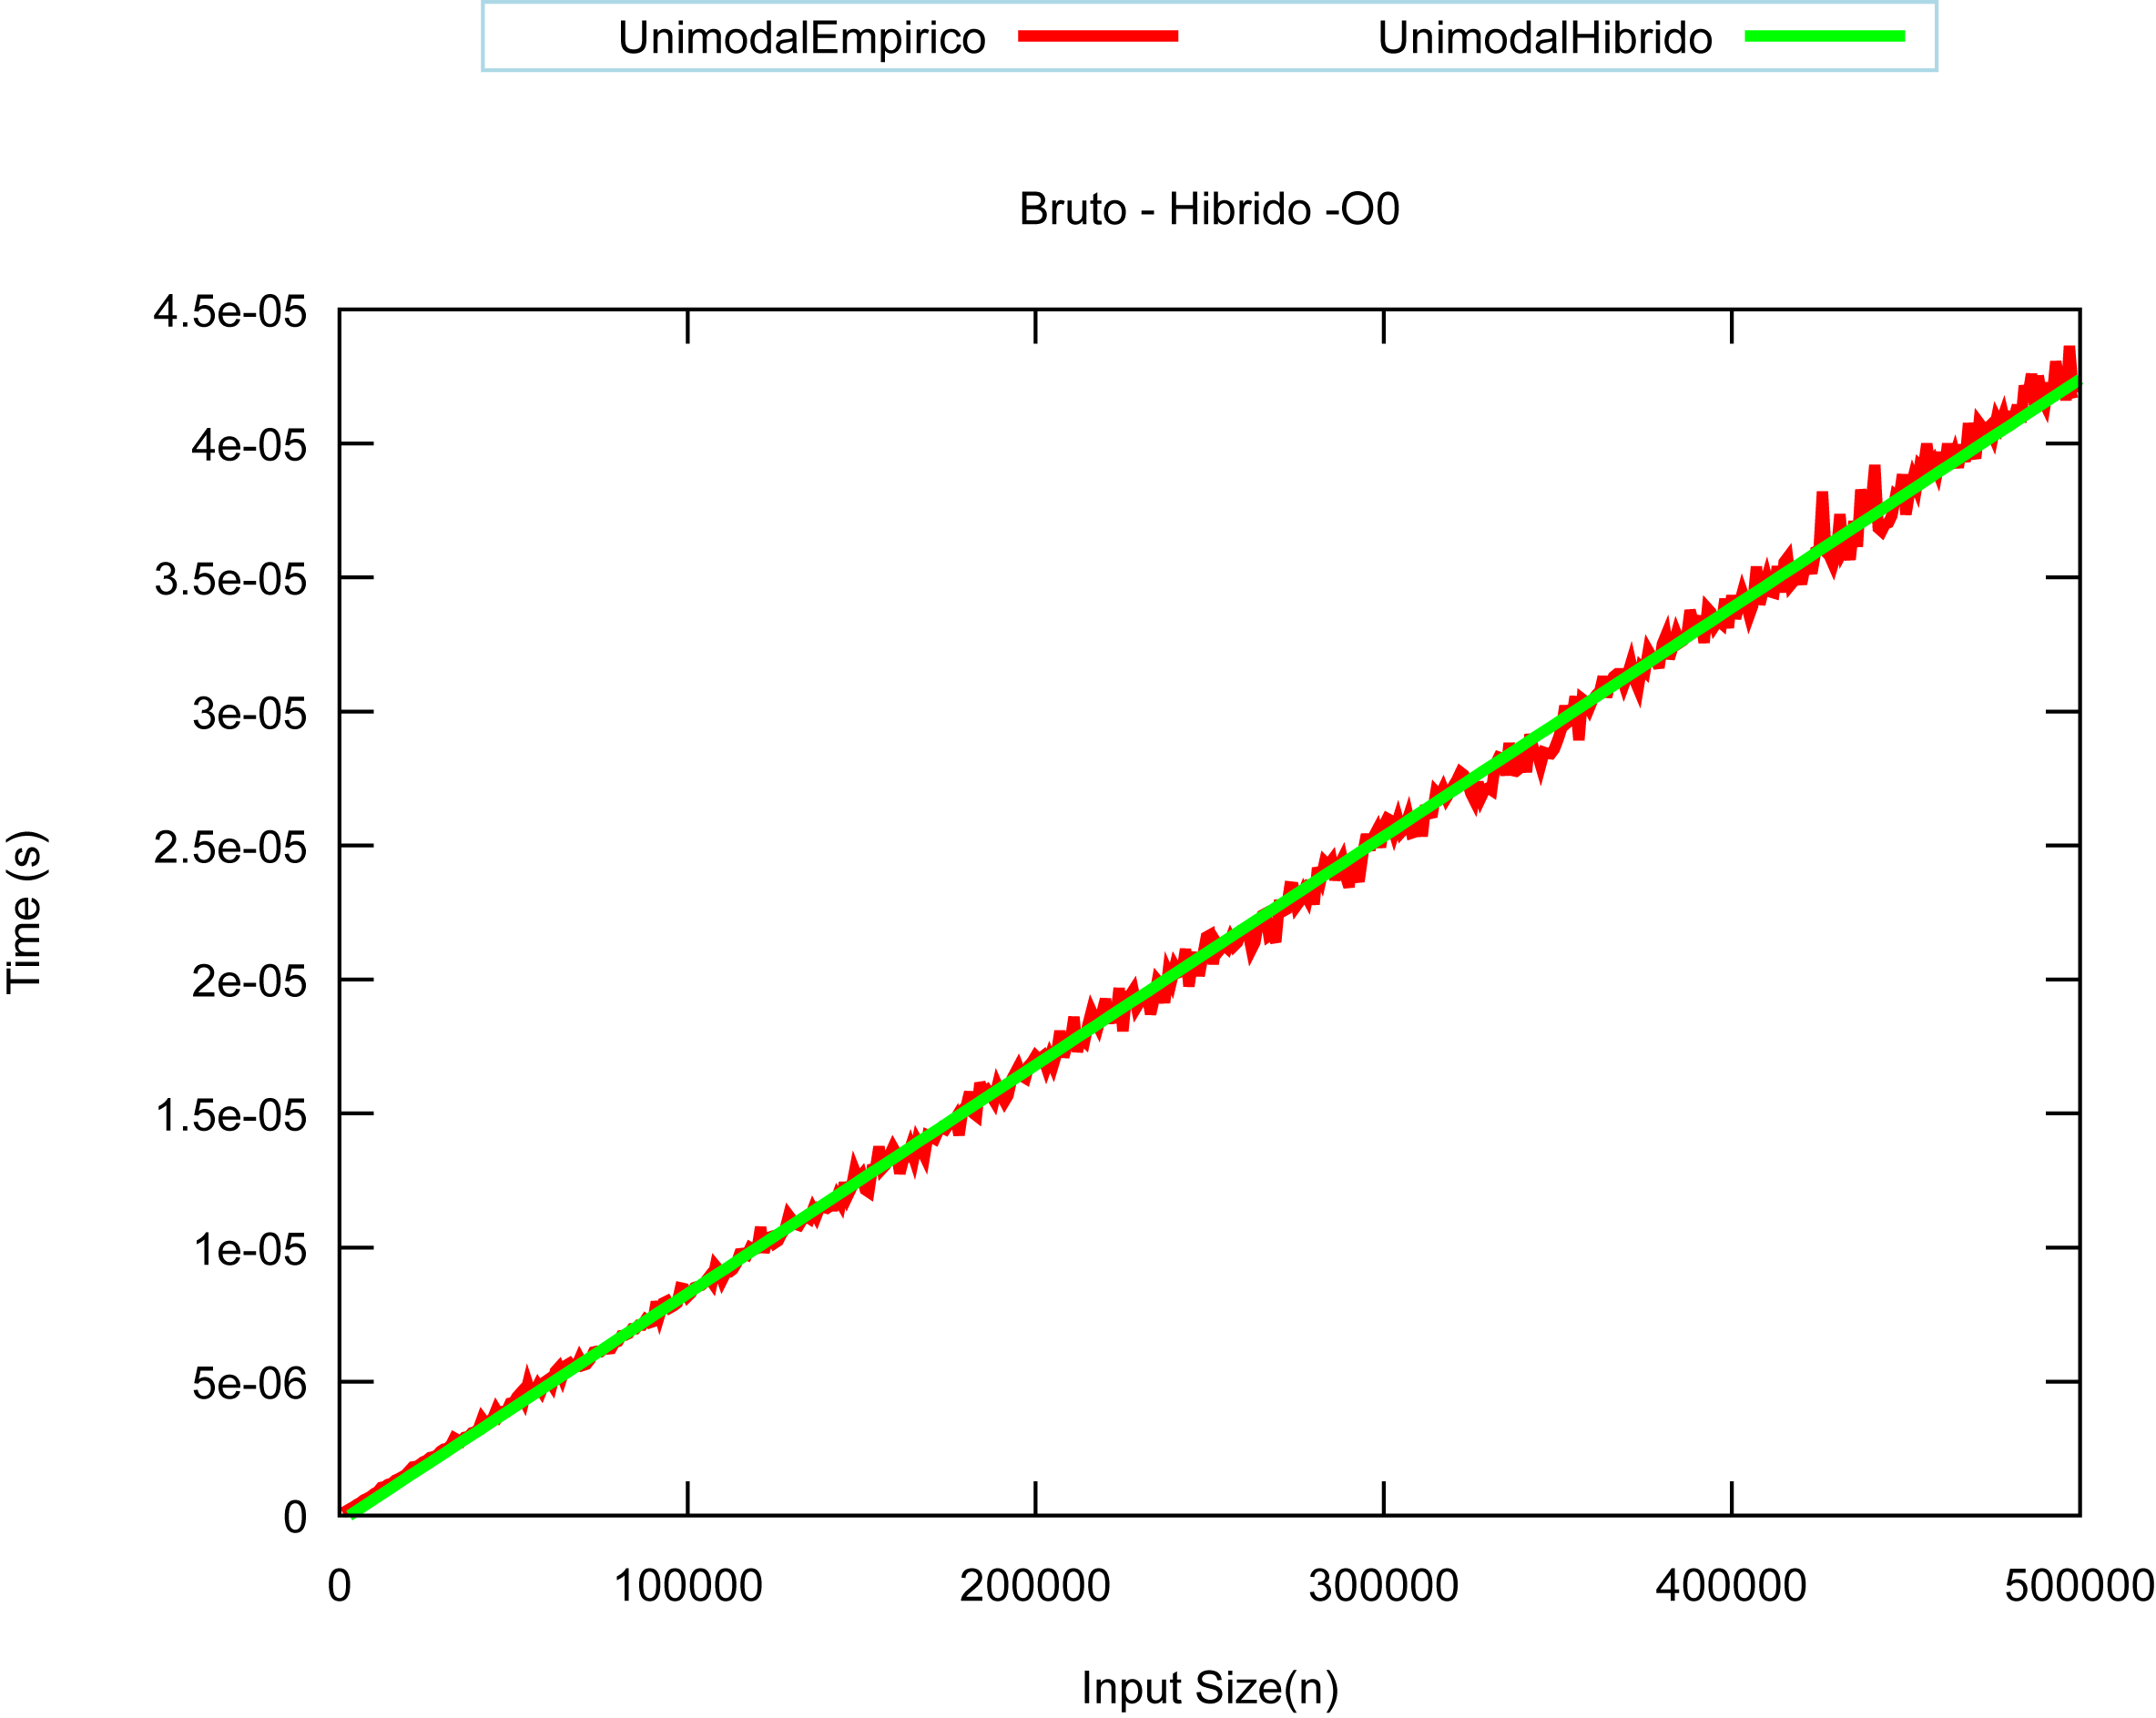
\includegraphics[width=8.6cm,height=7.1cm]{Images/bruto-hibridoO0}}
		\end{picture}
		\end{center}
		\end{figure}
		
\end{frame}	


	
\begin{frame}[plain]
	\frametitle{Constantes ocultas}
	
		\begin{defn}
			
			Sabemos que la función que describe la eficiencia de este algoritmo tiene la siguiente forma:
		\begin{equation}
			T(n)= a\cdot n + b
		\end{equation}
		
		Al realizar el ajuste de los datos con la herramienta \textit{gnuplot} obtenemos el valor de las constantes ocultas, quedando por tanto:
		
		\begin{equation}
			T(n) = 8.5281\cdot 10^{-11} \cdot n -2.43262\cdot 10^{-07}
		\end{equation}
	
		\vspace*{0.05in}
		
	\end{defn}
		
\end{frame}




\begin{frame}[plain]
	\frametitle{Optimización 1}
		\begin{figure}[htb]
		\begin{center}
		\begin{picture}(160,0)
		\put(-50,-110){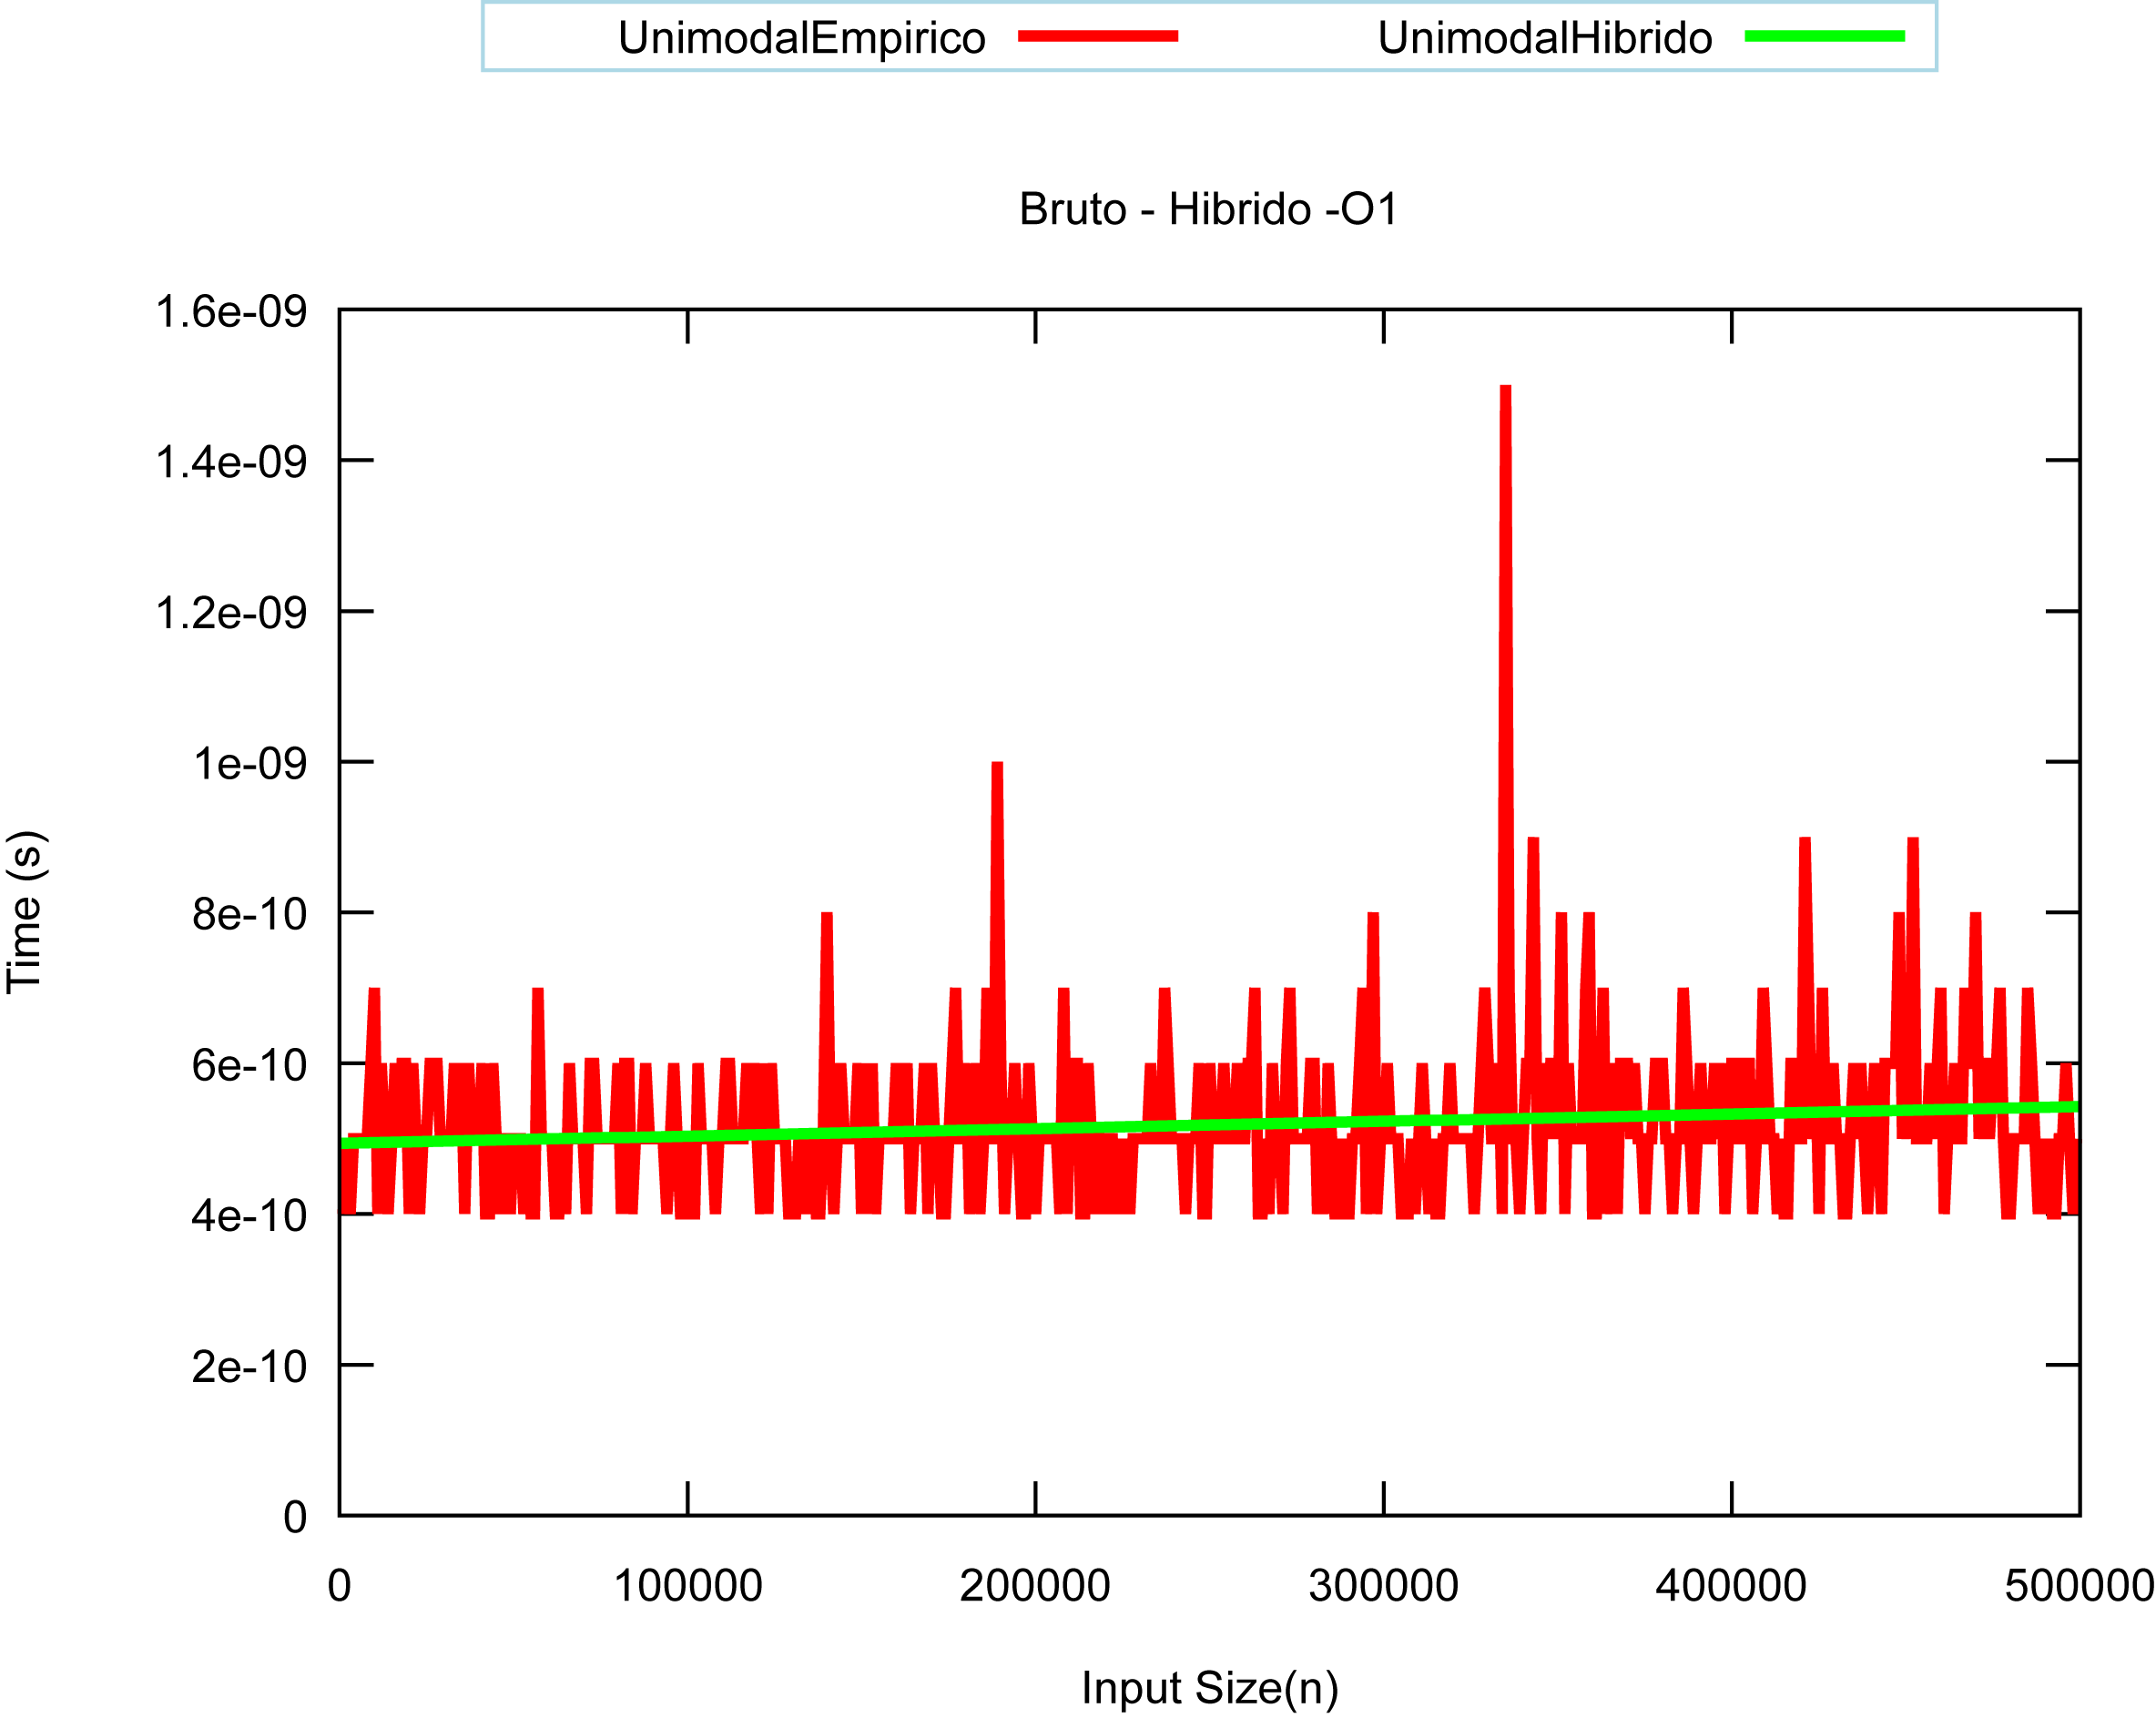
\includegraphics[width=8.6cm,height=7.1cm]{Images/bruto-hibridoO1}}
		\end{picture}
		\end{center}
		\end{figure}
		
\end{frame}	




\begin{frame}[plain]
	\frametitle{Constantes ocultas}
	
		\begin{defn}
			
			En este caso la función queda de la siguiente forma:
		
		\begin{equation}
			T(n) = 9.75348 \cdot 10^{-17} \cdot n + 4.93652 \cdot 10^{-07}
		\end{equation}
	
		\vspace*{0.05in}
		
	\end{defn}
	
	

		
\end{frame}














\begin{frame}[plain]
	\frametitle{Optimización 2}
		\begin{figure}[htb]
		\begin{center}
		\begin{picture}(160,0)
		\put(-50,-110){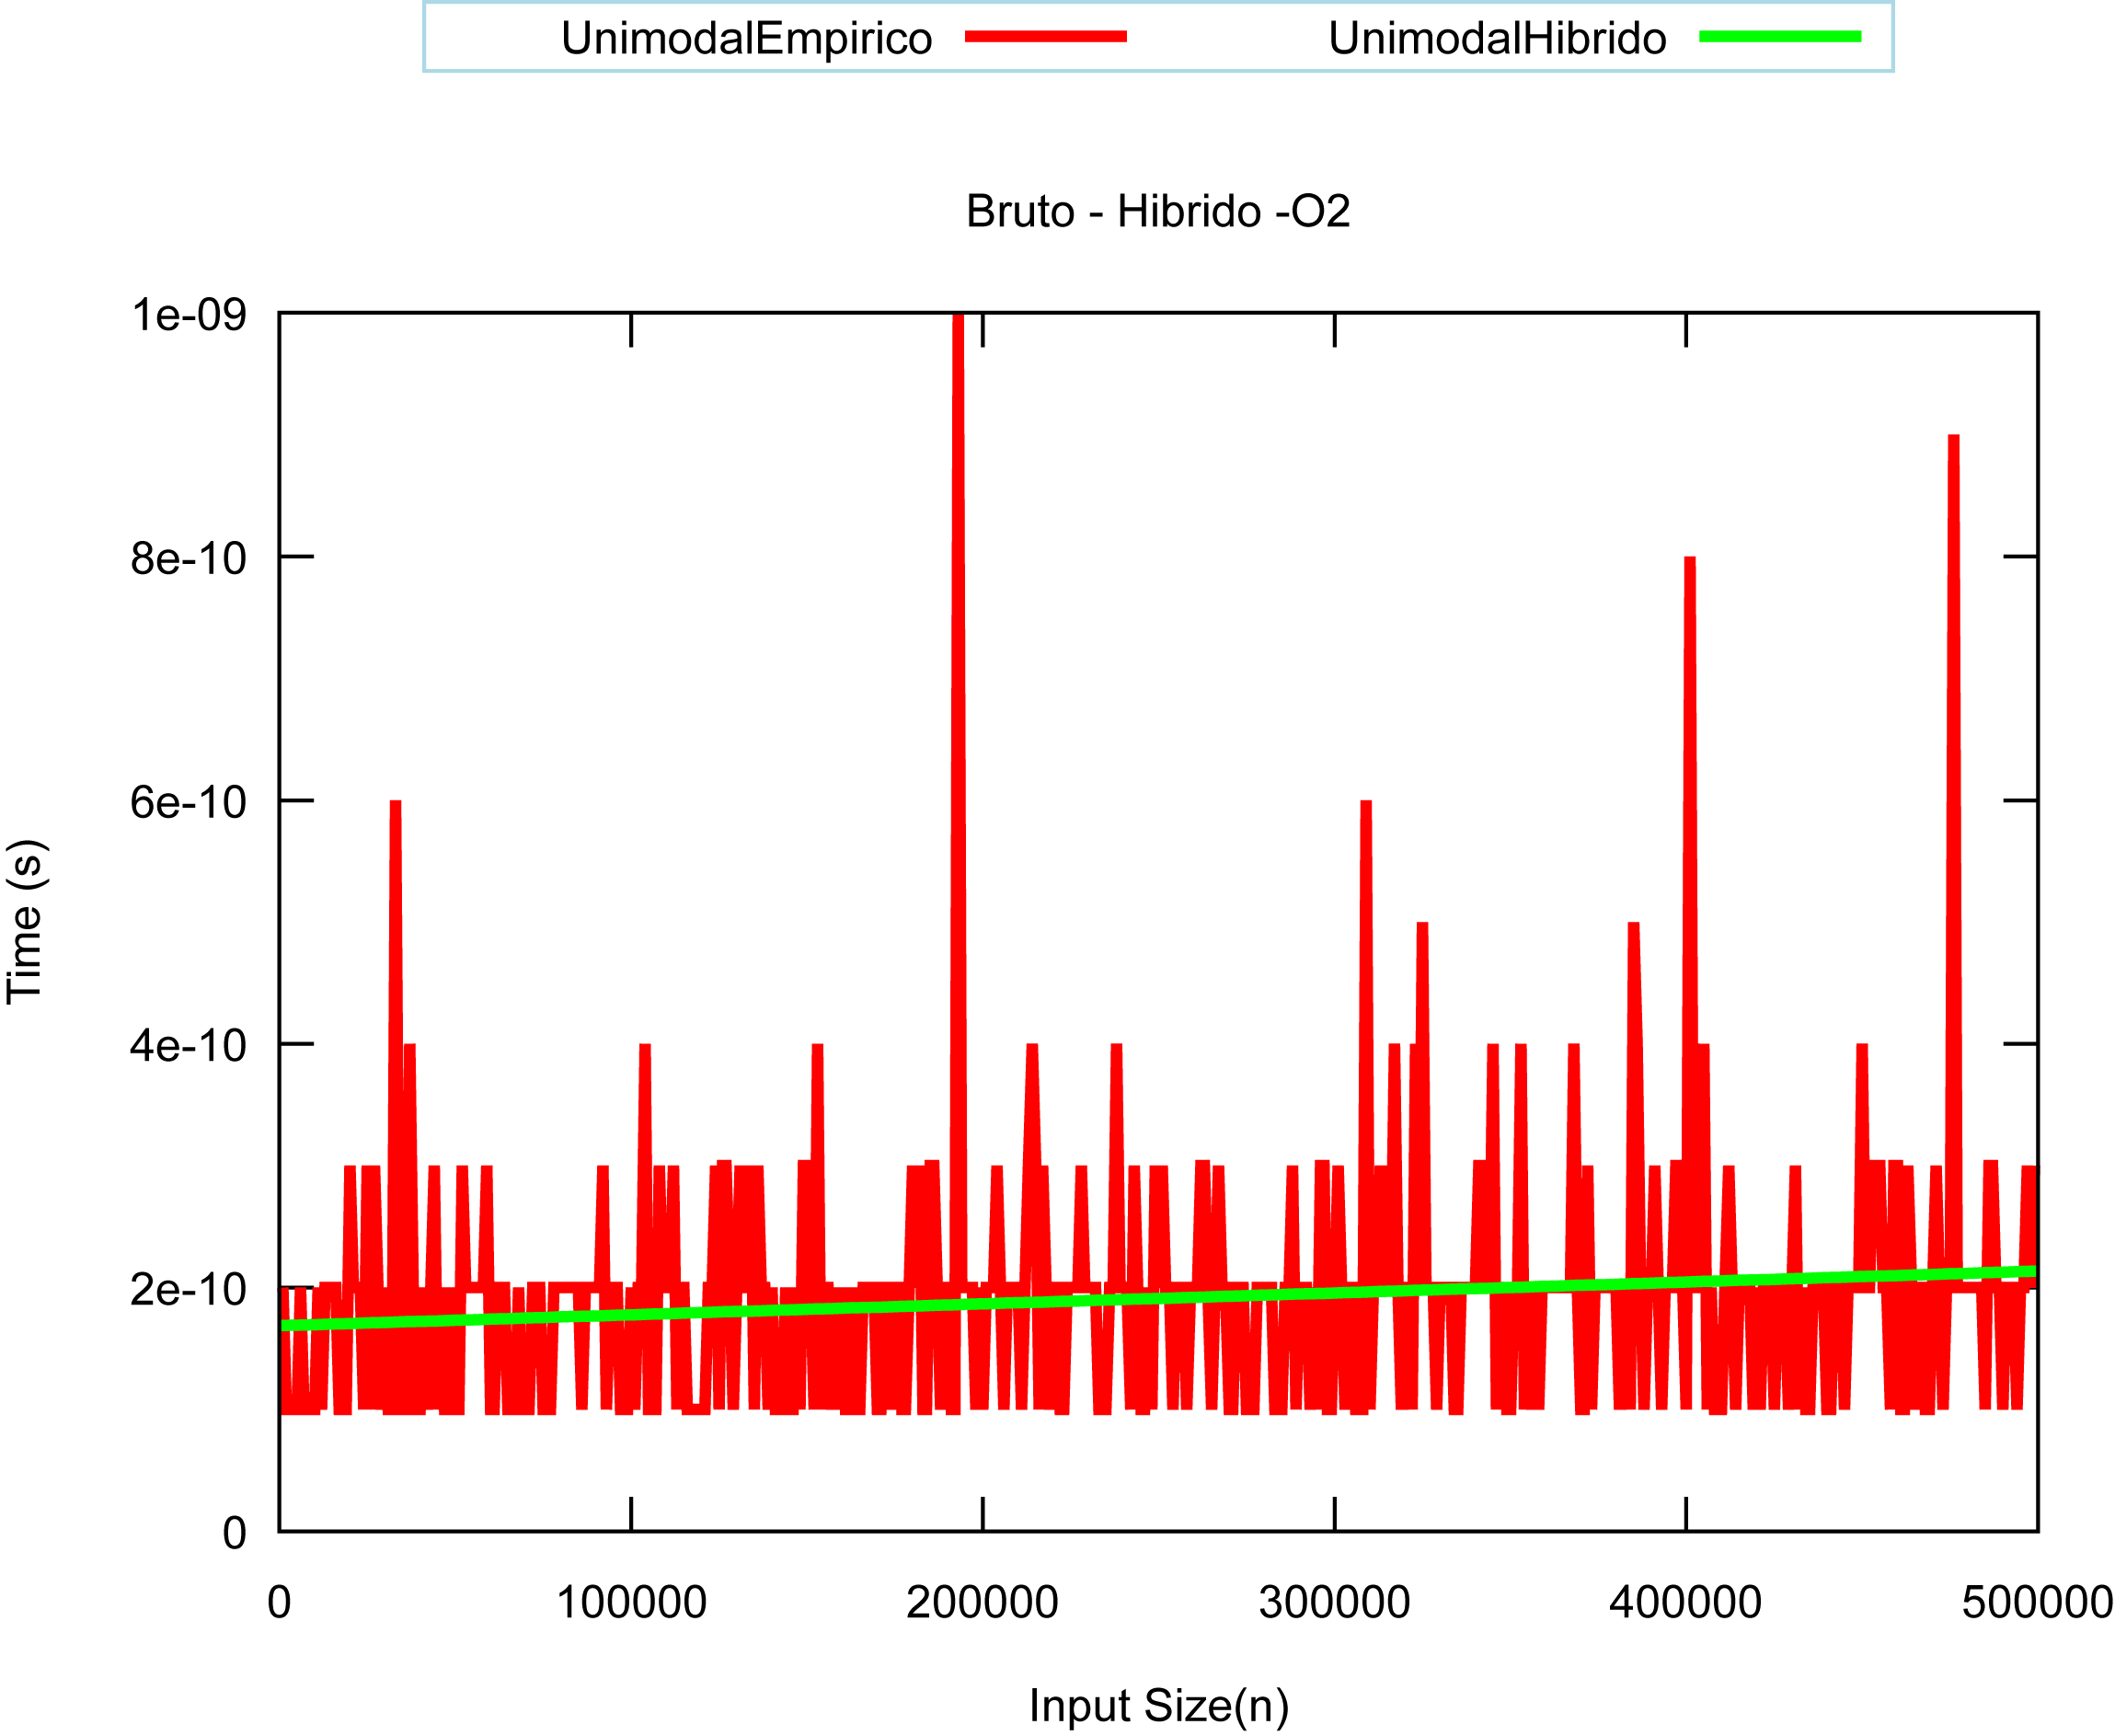
\includegraphics[width=8.6cm,height=7.1cm]{Images/bruto-hibridoO2}}
		\end{picture}
		\end{center}
		\end{figure}
		
\end{frame}	




\begin{frame}[plain]
	\frametitle{Constantes ocultas}
	
		\begin{defn}
			
			En este caso la función queda de la siguiente forma:
		
		\begin{equation}
			T(n) = 8.96154 \cdot 10^{-17} \cdot n + 1.68779 \cdot 10^{-07}
		\end{equation}
	
		\vspace*{0.05in}
		
	\end{defn}
	
	

		
\end{frame}




\begin{frame}[plain]
	\frametitle{Conclusión} 
	
	\begin{exampleblock}{Mejora}
			Como podemos ver, la mejora se encuentra en las constantes ocultas, concretamente, conseguimos una mejora muy sustancial en la pendiente, que pasamos de  $a= 8.5281\cdot 10^{-11}$ a $a =  9.75348e\cdot 10^{-17}$
		\end{exampleblock}
\end{frame}		

		
		
		
		
		
	




	\section[Algoritmo Divide y Vencerás]{Algoritmo Divide y Vencerás}
\begin{frame}[plain]
	\frametitle{Resolución}
		\begin{exampleblock}{Estrategia de resolución}
			Nos posicionamos sobre el elemento que ocupa la posición media de la estructura:
			\begin{enumerate}
				\item  Si el elemento a su izquierda es mayor y si elemento a la derecha es menor, entonces, nos quedamos con la primera mitad de la estructura.
				\item Si el elemento a su izquierda es menor y su elemento a la derecha es mayor, entonces, nos quedamos con la segunda mitad de la estructura.
				\item Si el elemento a su izquierda es menor y su elemento a la derecha es menor: ¡Hemos encontrado el elemento que buscábamos!
			\end{enumerate}
		\end{exampleblock}
		
\end{frame}		




\begin{frame}[plain]
	\frametitle{Breve explicación - Paso 0}
		\begin{figure}[htb]
		\begin{center}
		\begin{picture}(160,0)
		\put(-110,-100){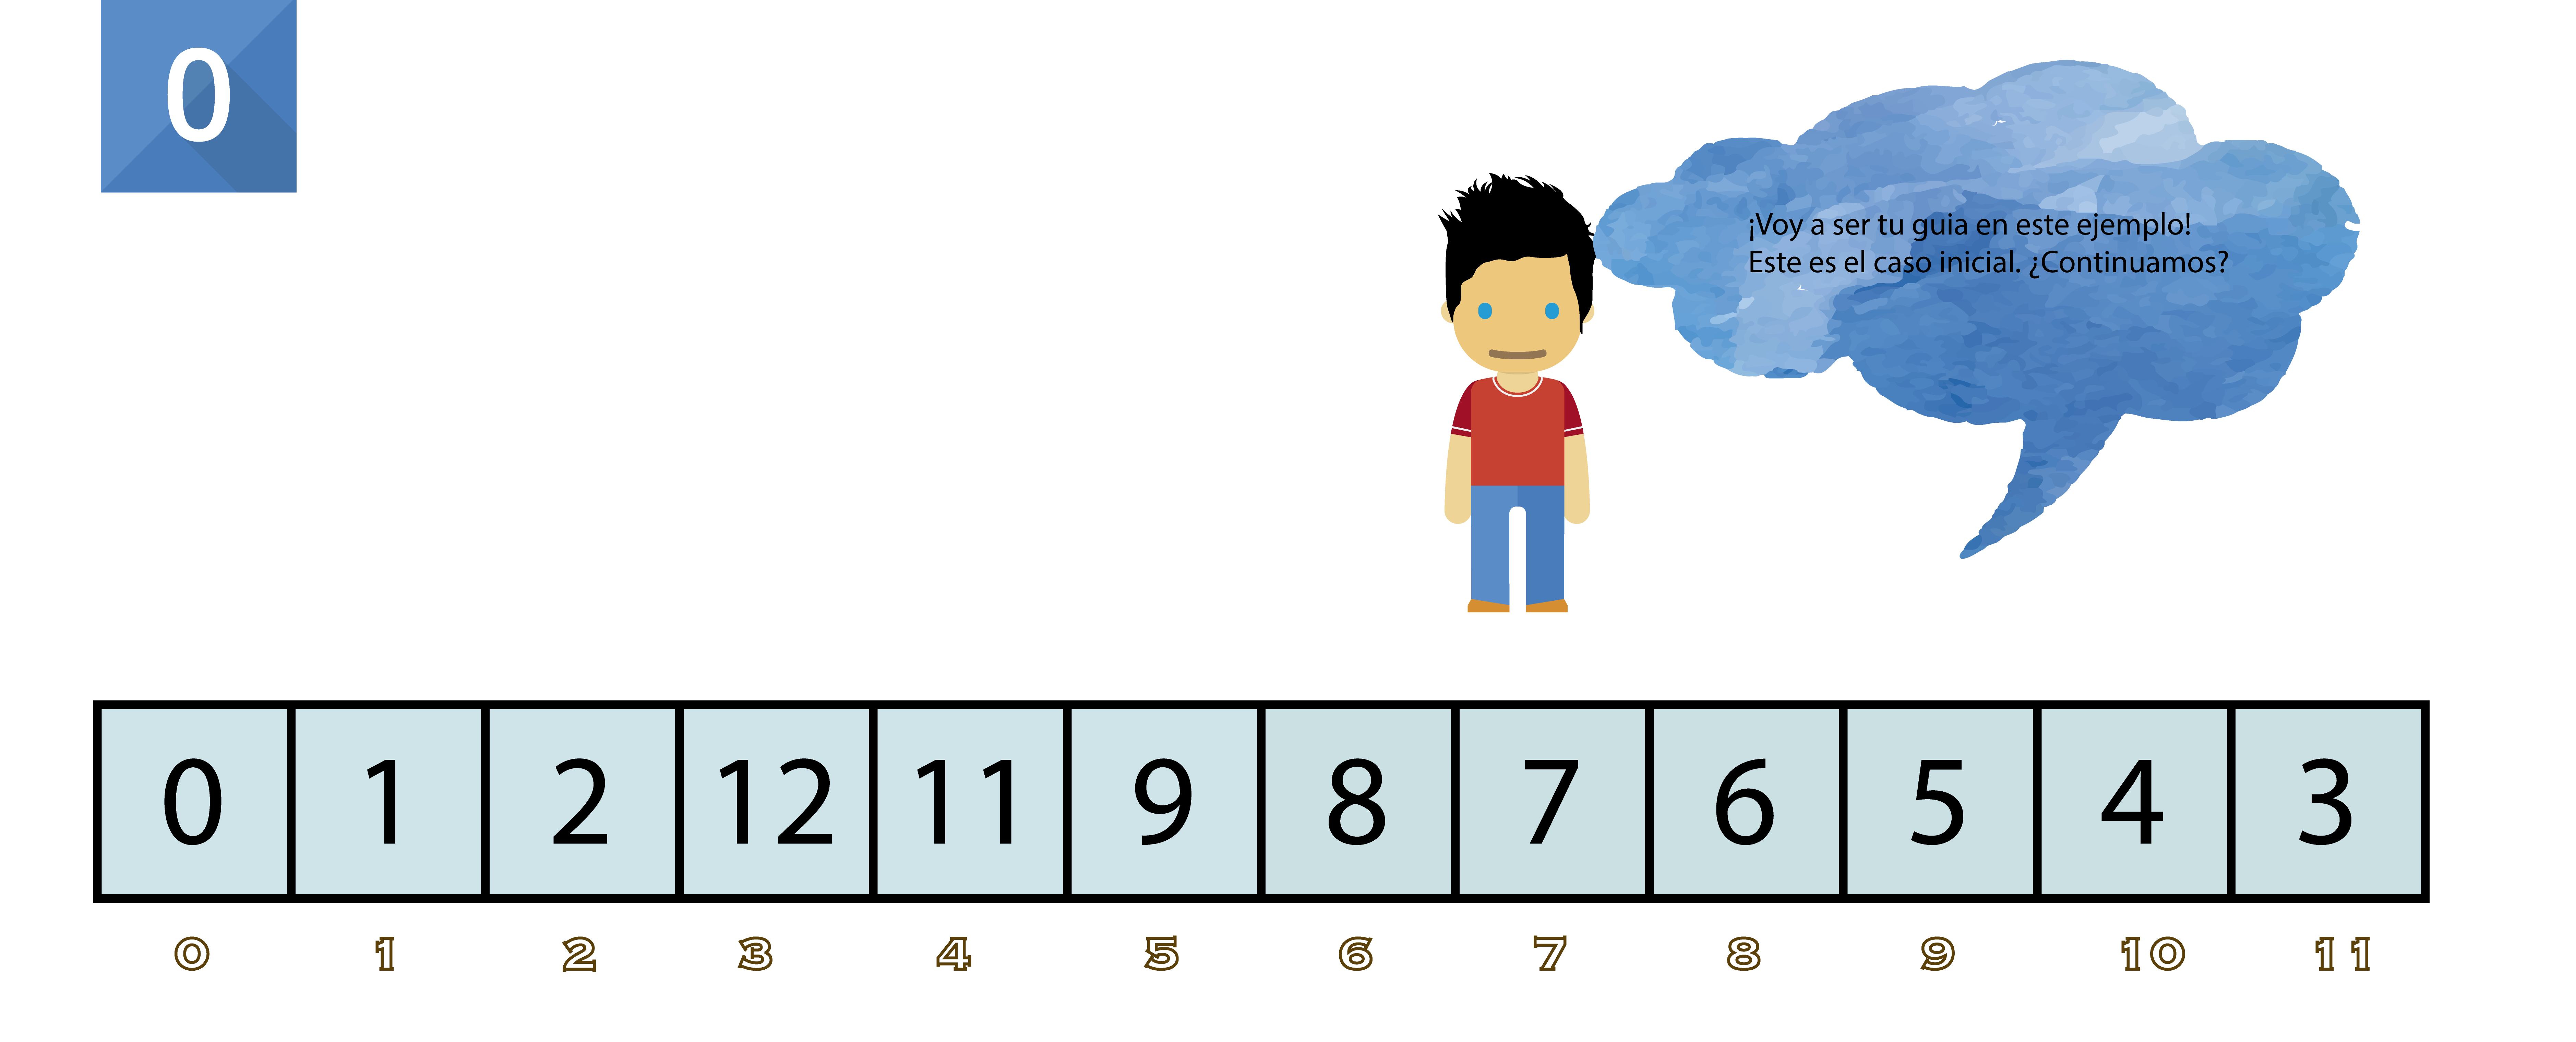
\includegraphics[width=13.5cm,height=6.5cm]{Images/Paso0}}
		\end{picture}
		\end{center}
		\end{figure}
		
\end{frame}	

\begin{frame}[plain]
	\frametitle{Breve explicación - Paso 1}
		\begin{figure}[htb]
		\begin{center}
		\begin{picture}(160,0)
		\put(-110,-100){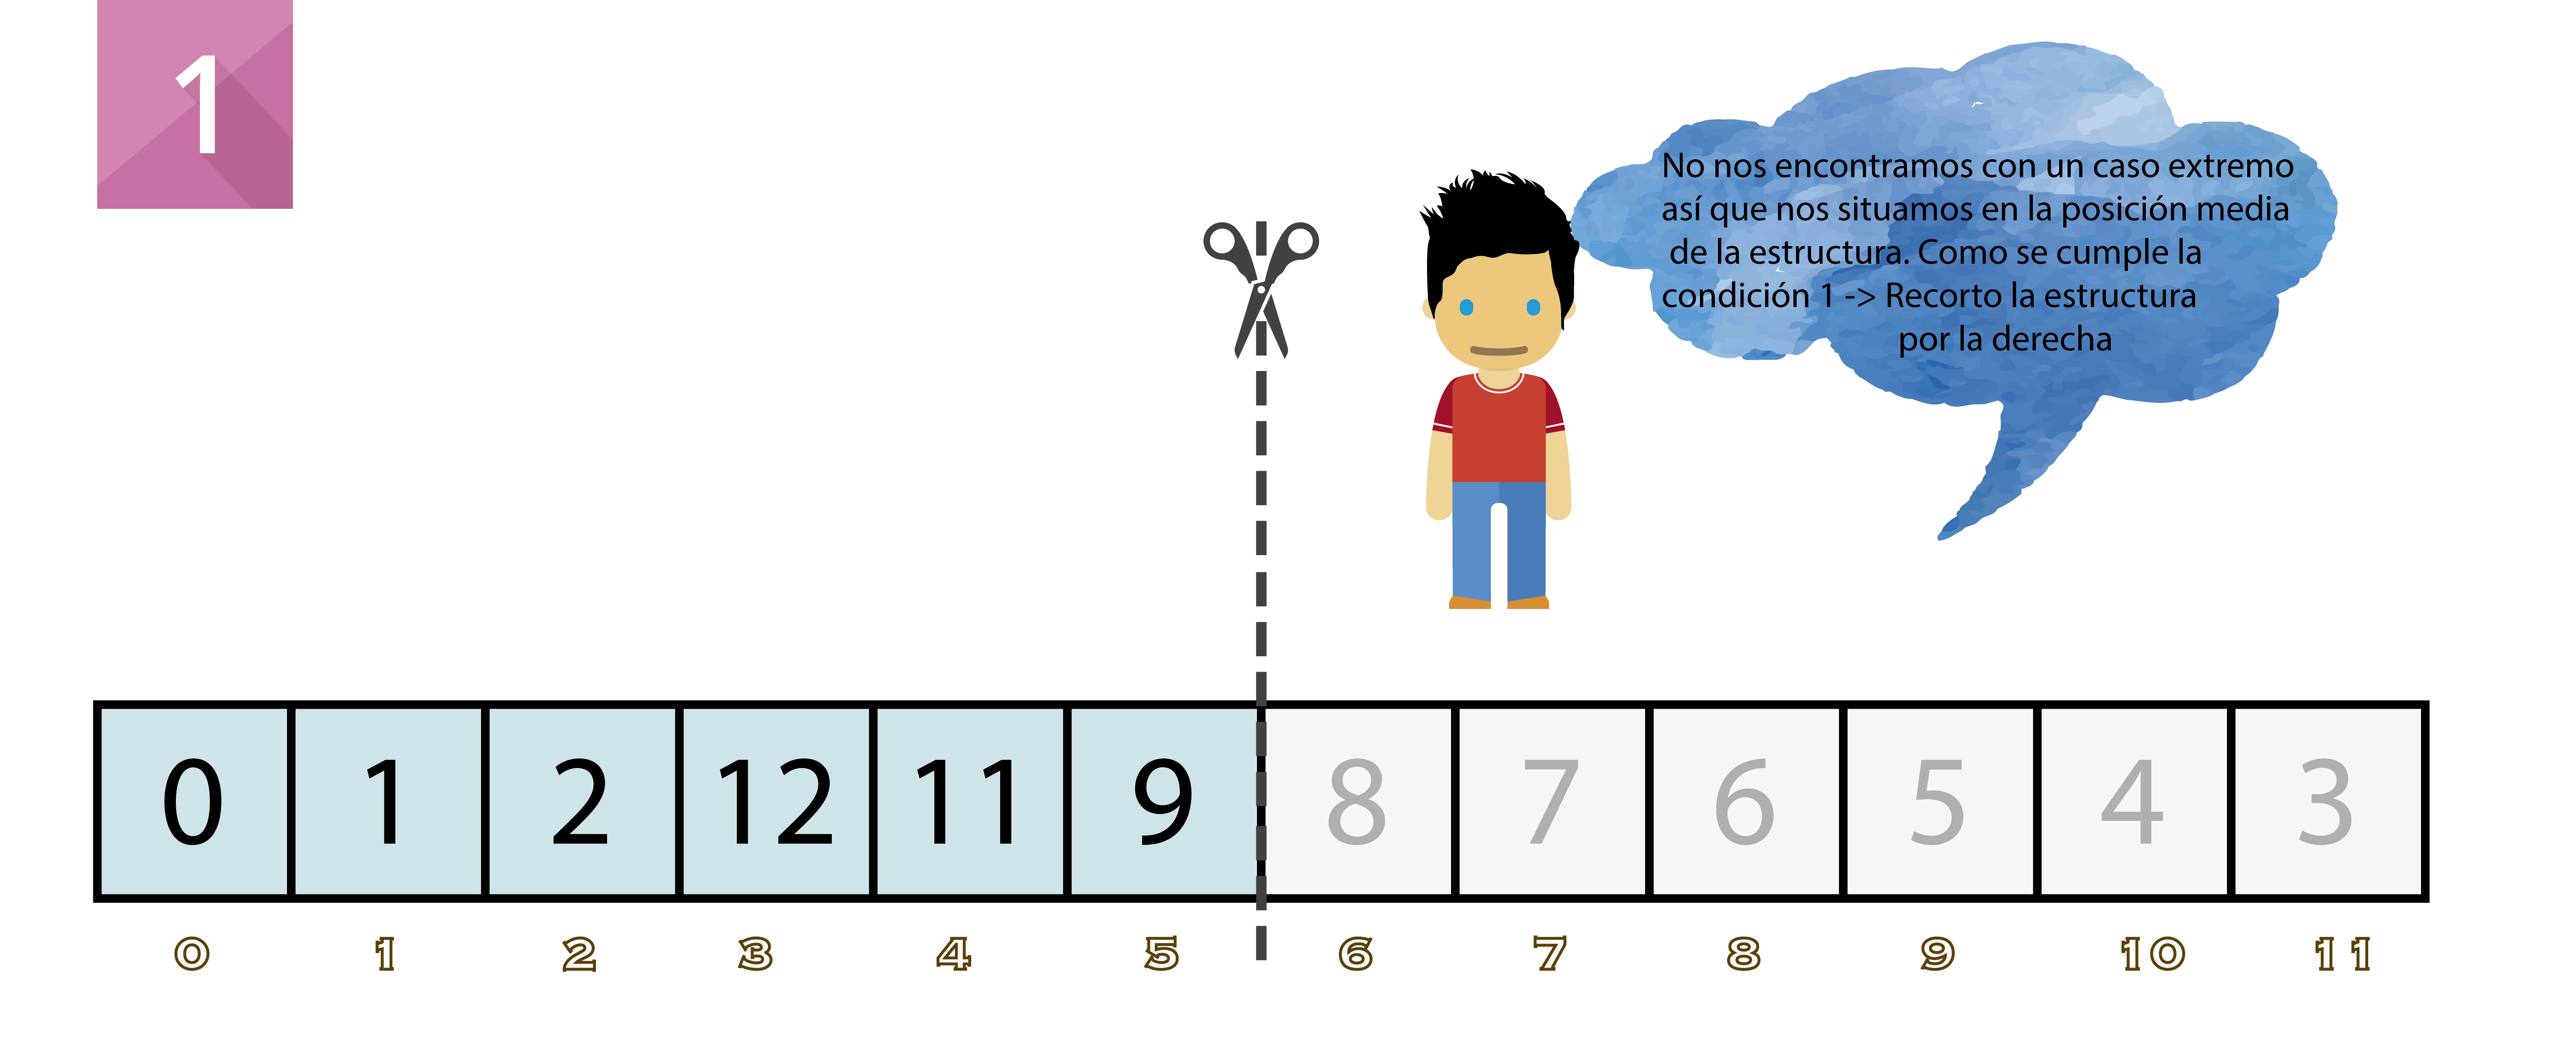
\includegraphics[width=13.5cm,height=6.5cm]{Images/Paso1}}
		\end{picture}
		\end{center}
		\end{figure}
		
\end{frame}	

\begin{frame}[plain]
	\frametitle{Breve explicación - Paso 2}
		\begin{figure}[htb]
		\begin{center}
		\begin{picture}(160,0)
		\put(-110,-100){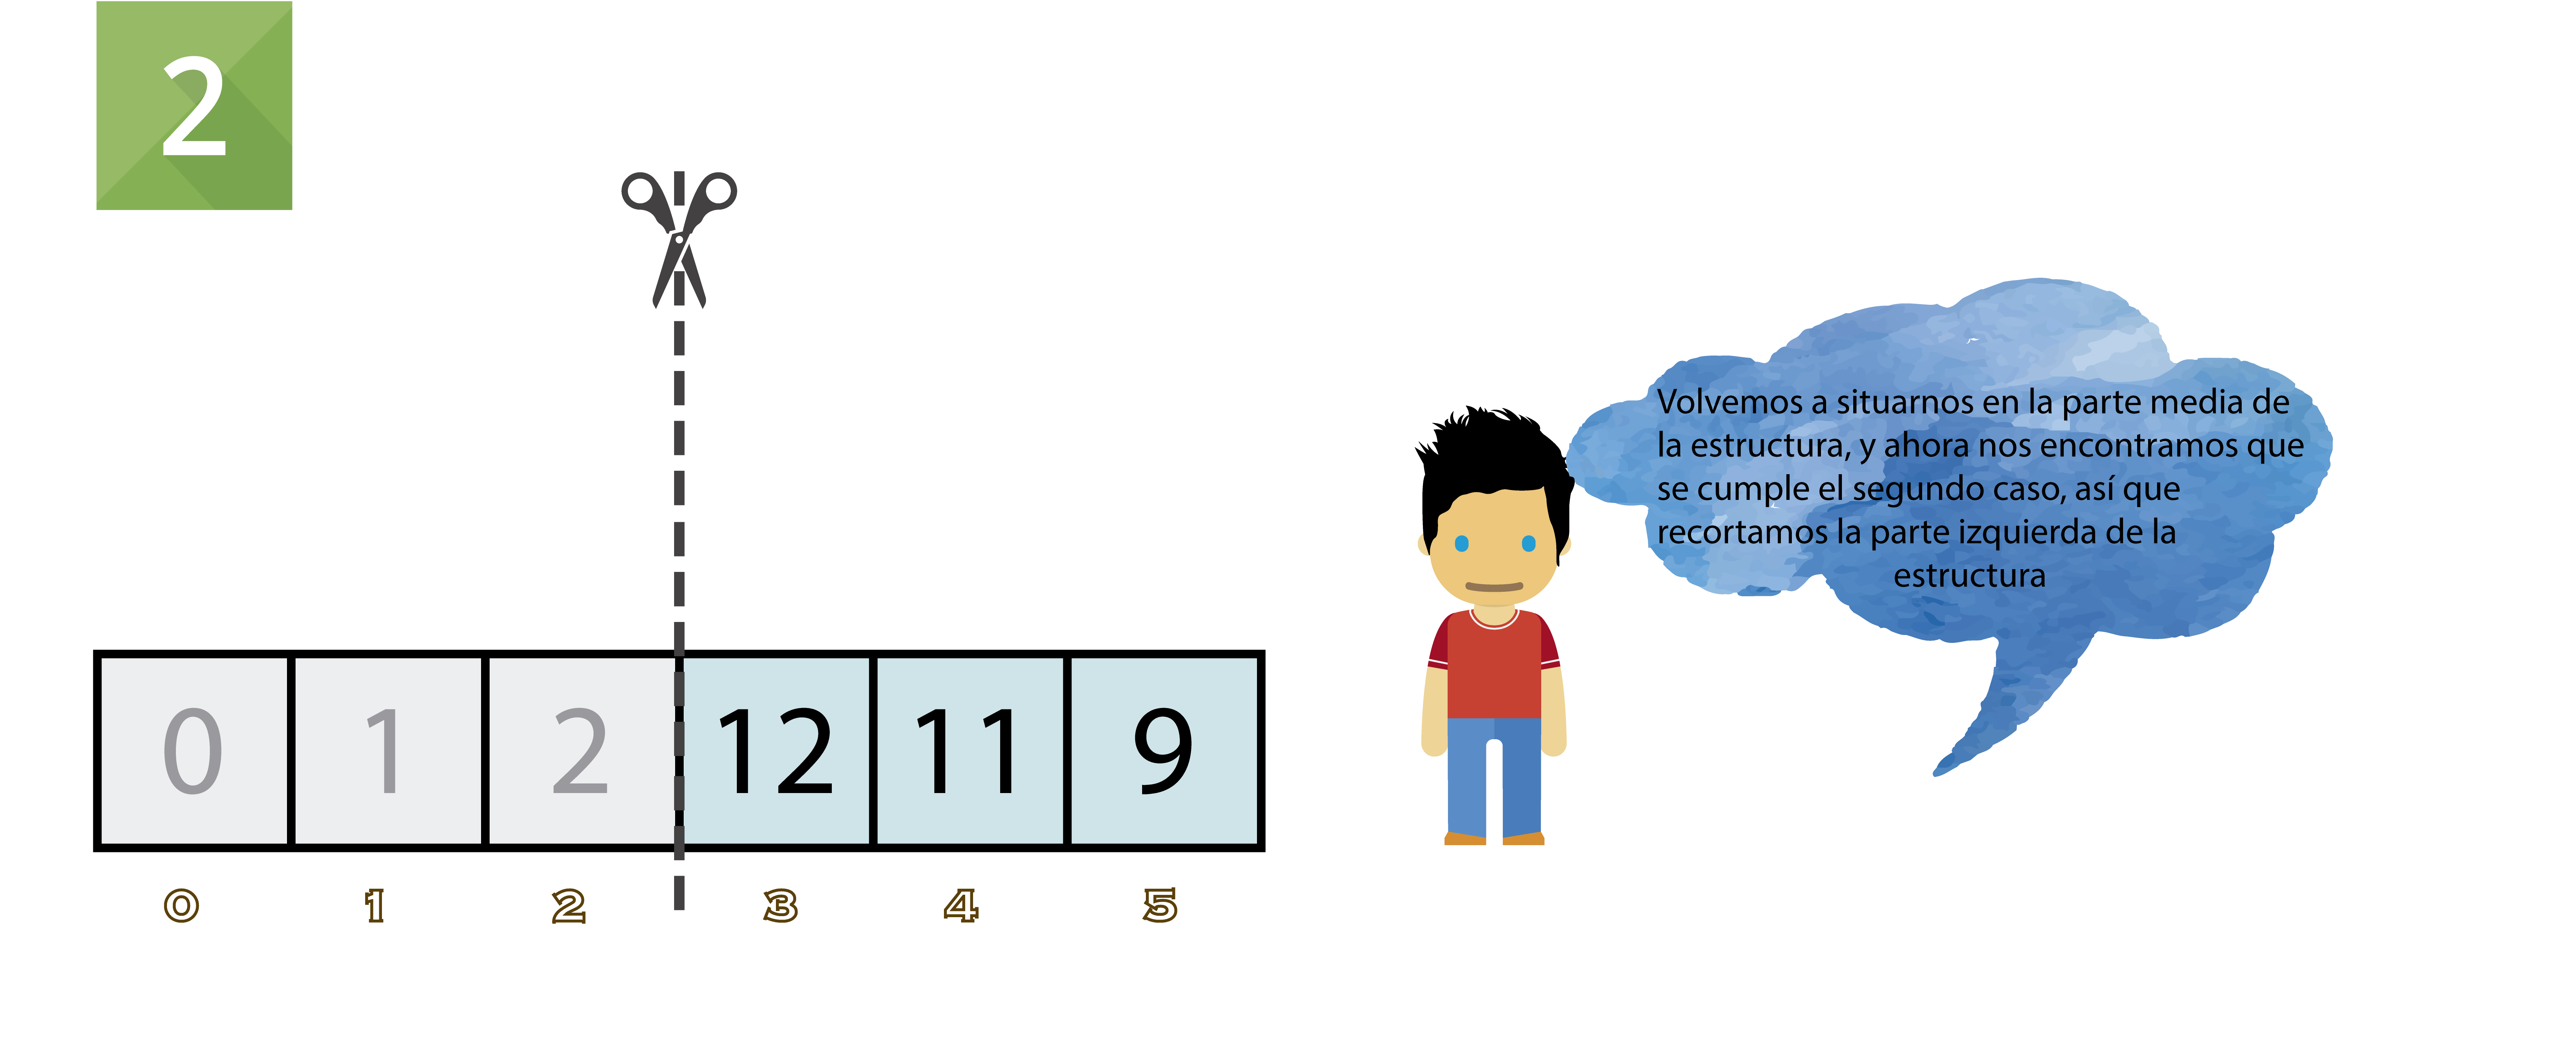
\includegraphics[width=13.5cm,height=6.5cm]{Images/Paso2}}
		\end{picture}
		\end{center}
		\end{figure}
		
\end{frame}	

\begin{frame}[plain]
	\frametitle{Breve explicación - Paso 3}
		\begin{figure}[htb]
		\begin{center}
		\begin{picture}(160,0)
		\put(-110,-100){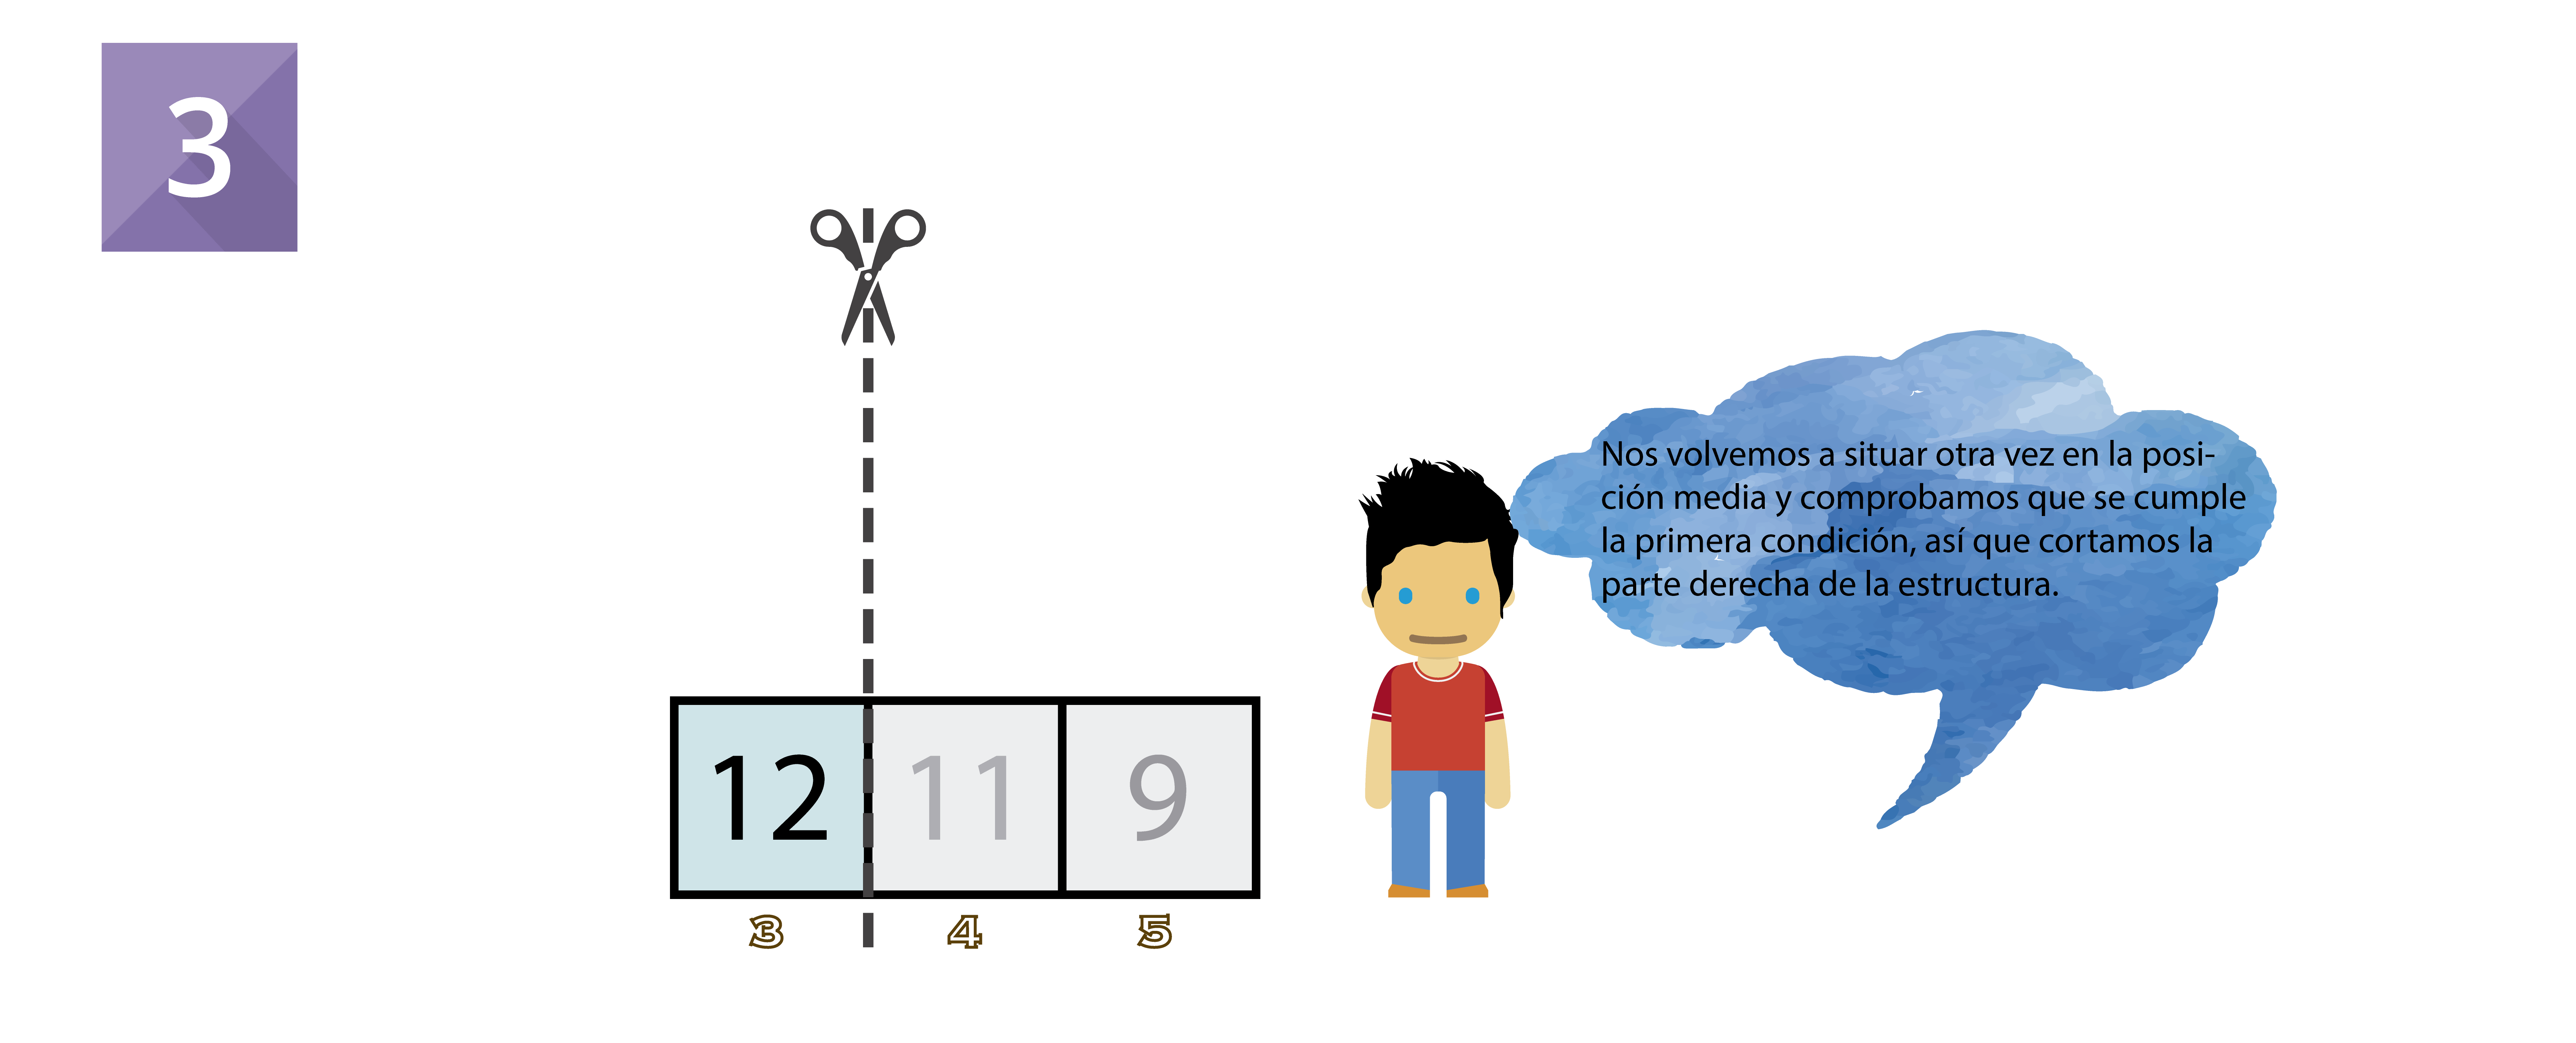
\includegraphics[width=13.5cm,height=6.5cm]{Images/Paso3}}
		\end{picture}
		\end{center}
		\end{figure}
		
\end{frame}	

\begin{frame}[plain]
	\frametitle{Breve explicación - Paso 4}
		\begin{figure}[htb]
		\begin{center}
		\begin{picture}(160,0)
		\put(-110,-100){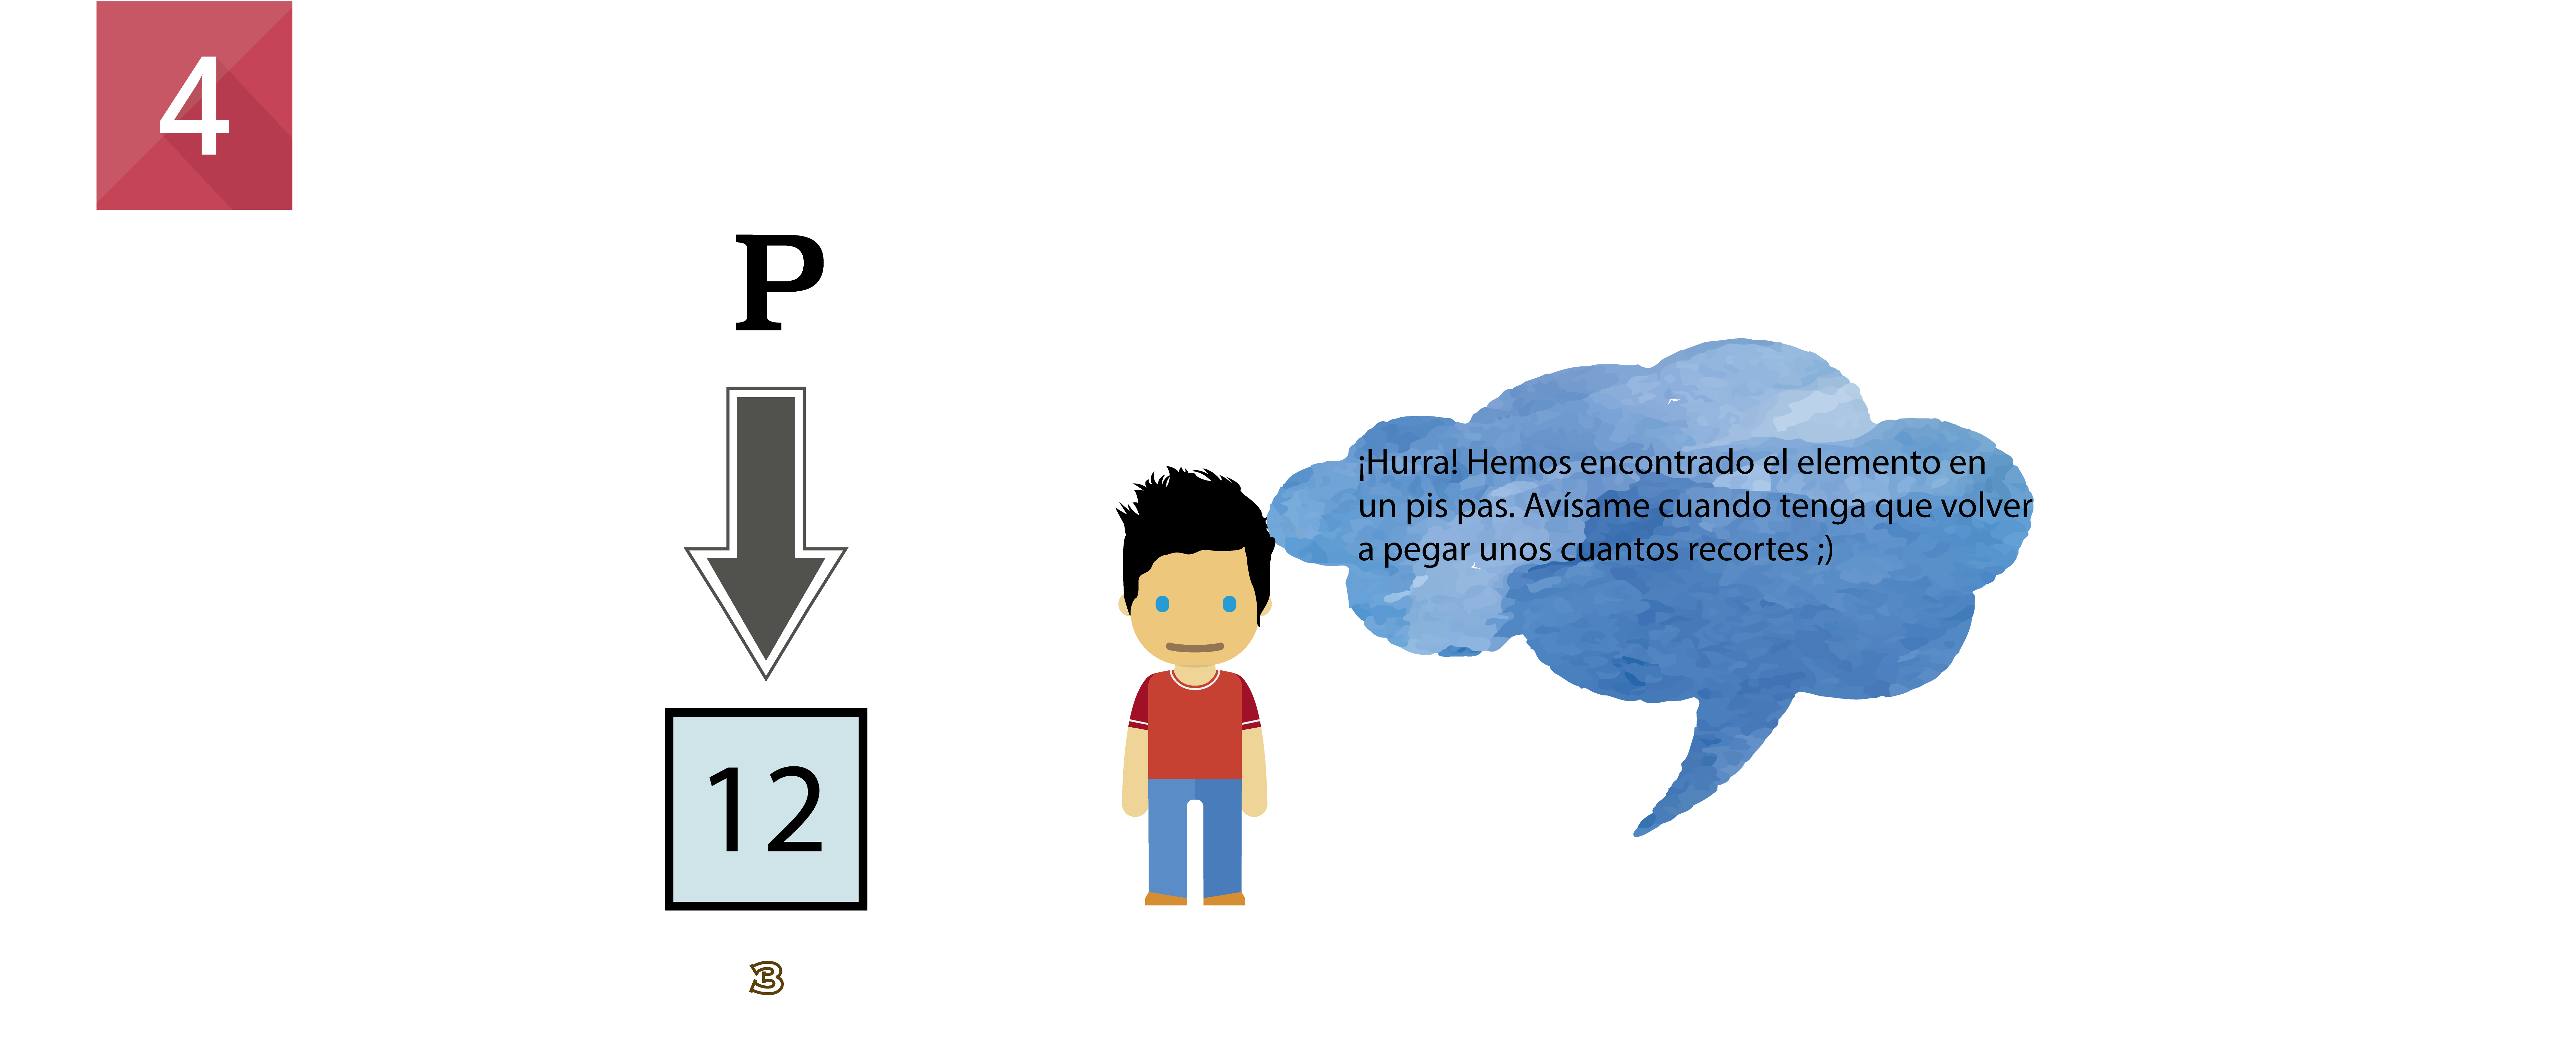
\includegraphics[width=13.5cm,height=6.5cm]{Images/Paso4}}
		\end{picture}
		\end{center}
		\end{figure}
		
\end{frame}	









\begin{frame}[fragile]
	\frametitle{Algoritmo Bruto - Implementación}
	\lstset{language=C++,
                basicstyle=\ttfamily,
                tabsize=3, 
				showstringspaces=false,
				extendedchars=true,
                keywordstyle=\color{blue}\ttfamily,
                stringstyle=\color{red}\ttfamily,
                commentstyle=\color{yellow}\ttfamily,
                basicstyle=\small,
                morecomment=[l][\color{magenta}]{\#}
     }
			\vspace*{-0.1in}
\begin{lstlisting}
int unimodalDyV(vector<int> &v, int inicio, int final){
    int posicionMedia = (inicio + final) / 2;
    bool found = false;
    if(posicionMedia > inicio){
        if(v[posicionMedia-1] > v[posicionMedia] 
        && v[posicionMedia] > v[posicionMedia+1])
             return unimodalDyV(v, inicio, posicionMedia);
        else if(v[posicionMedia-1] < v[posicionMedia] 
        		&& v[posicionMedia] < v[posicionMedia+1])
            return unimodalDyV(v, posicionMedia, final);
        else if(v[posicionMedia] > v[posicionMedia-1] 
        		&& v[posicionMedia+1]<v[posicionMedia])
            return posicionMedia;
    }else{
        if(v[inicio] <= v[final])
            return final;
        else
            return inicio;
    }
}

\end{lstlisting}		
\end{frame}	


\begin{frame}[plain]
	\frametitle{Análisis Híbrido}
		\begin{figure}[htb]
		\begin{center}
		\begin{picture}(160,0)
		\put(-50,-110){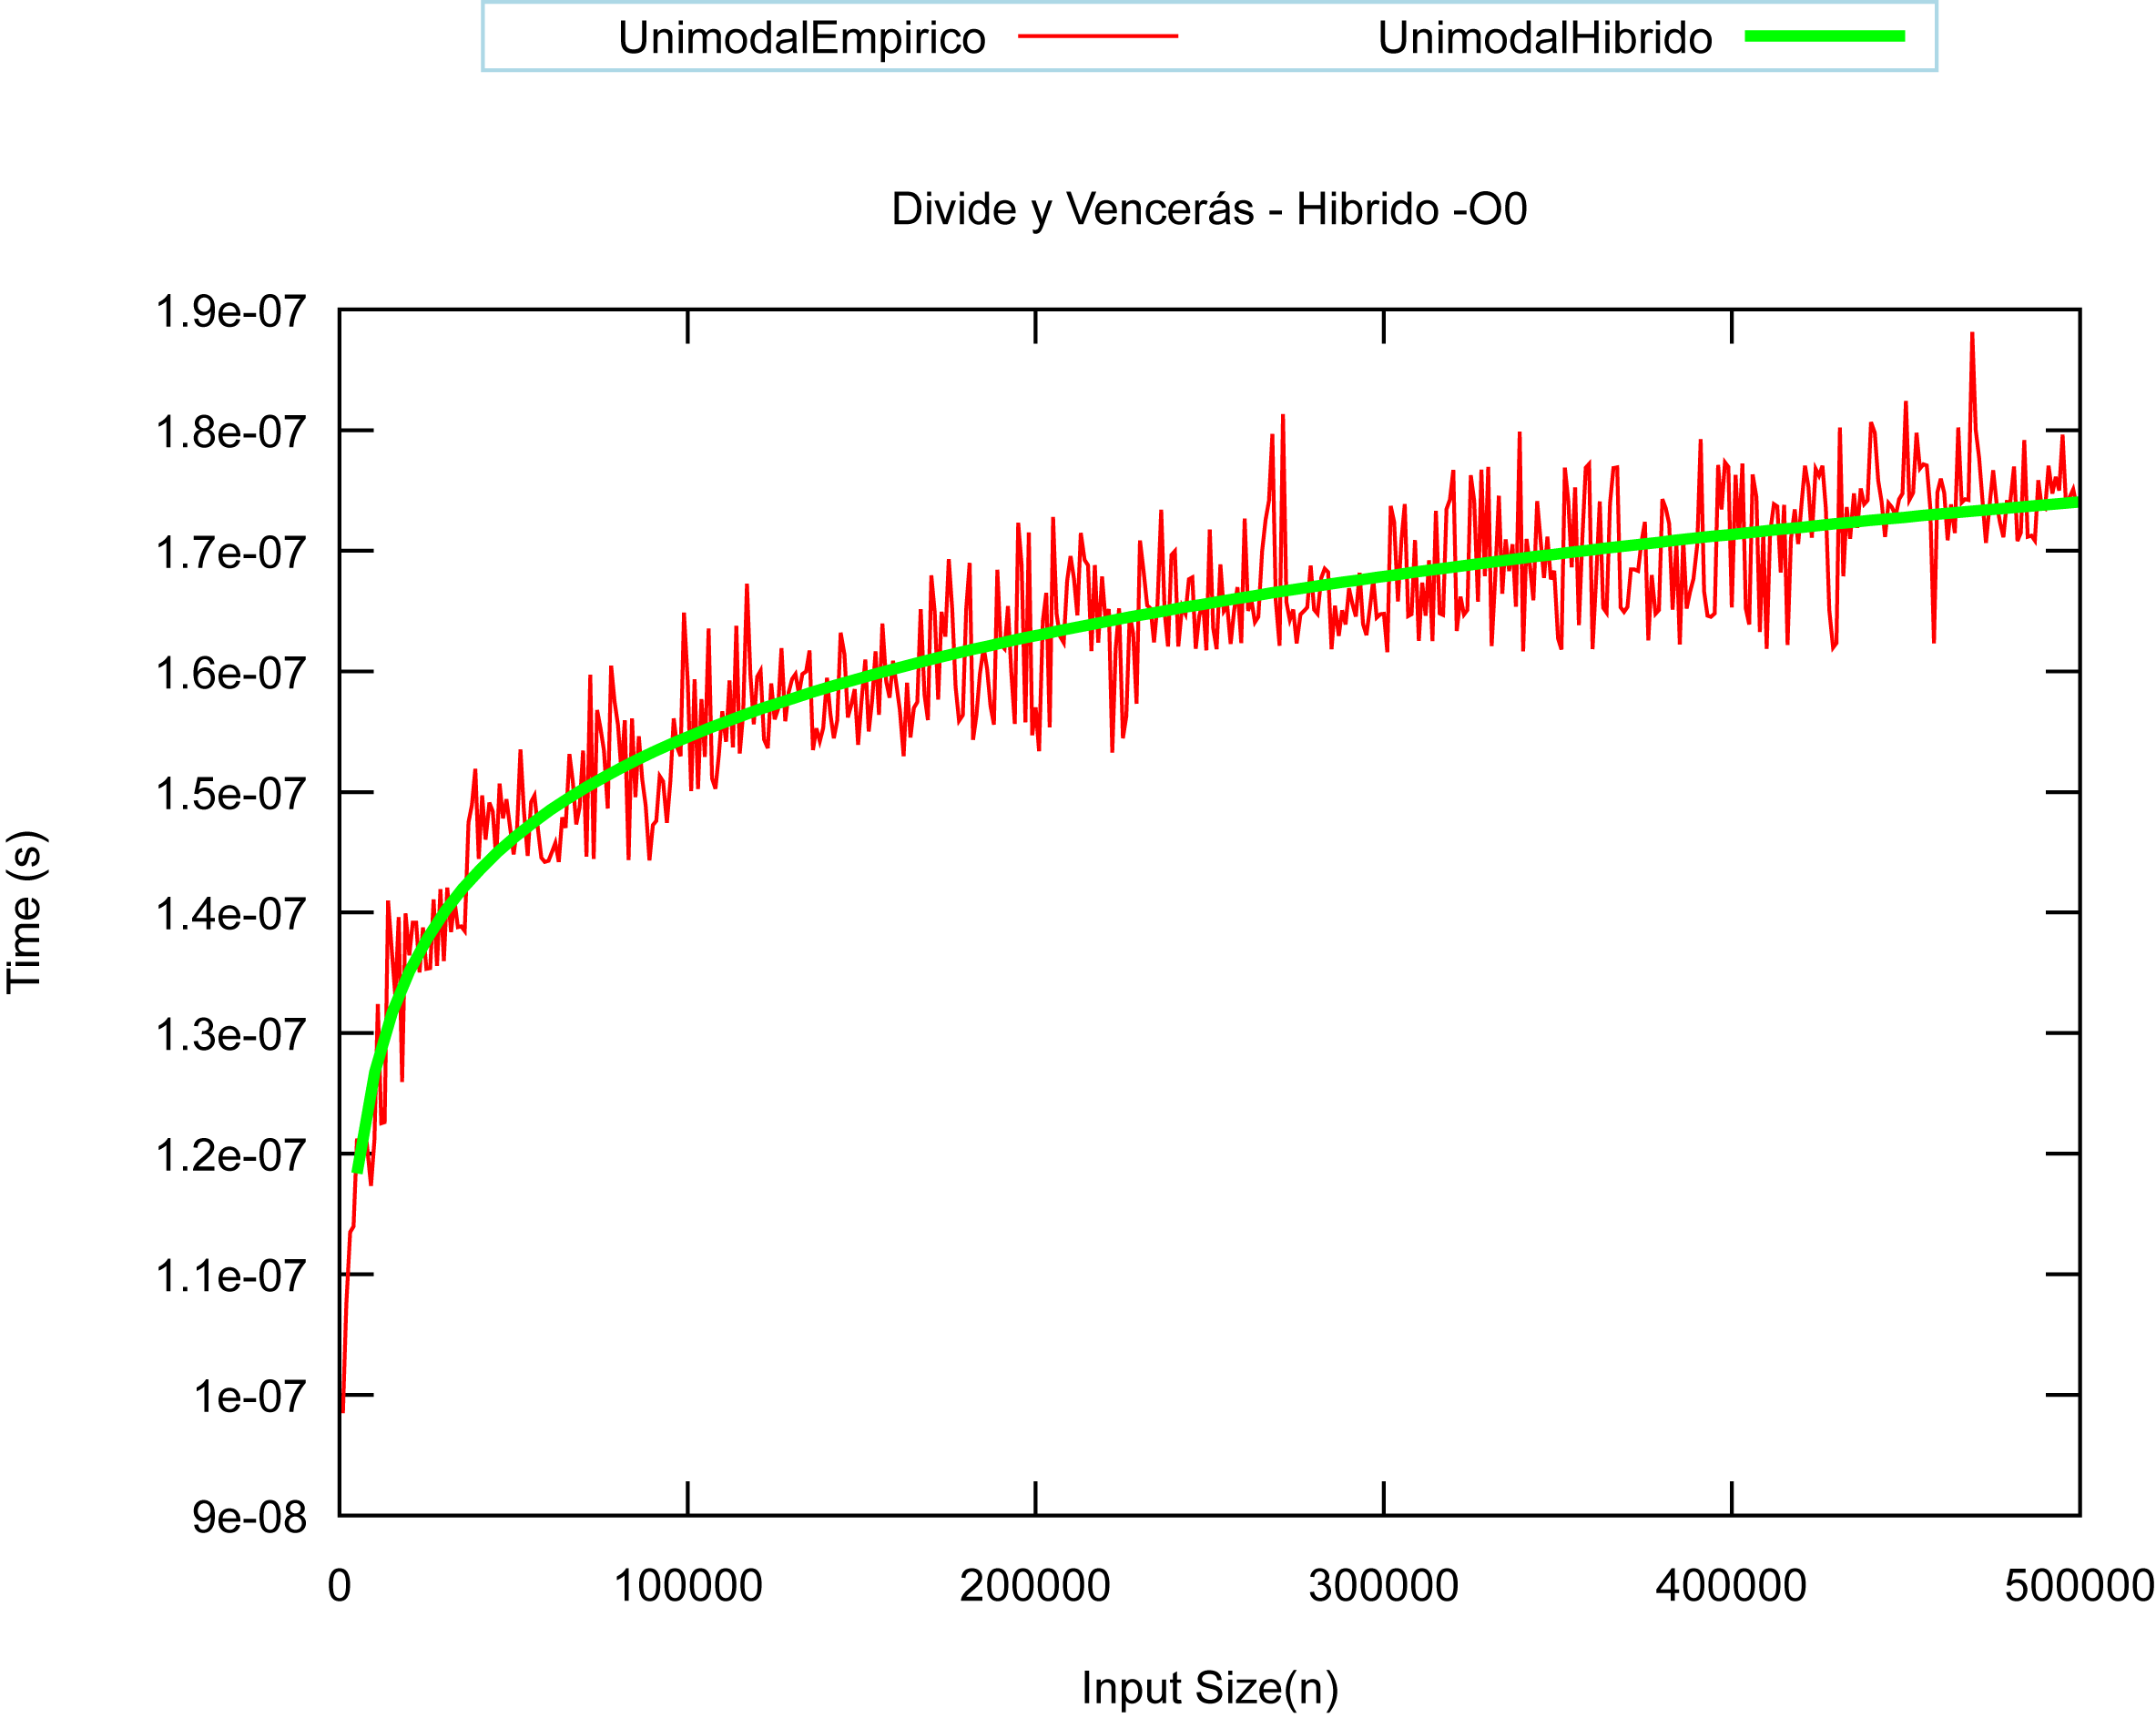
\includegraphics[width=8.6cm,height=7.1cm]{Images/dyv-hibridoO0}}
		\end{picture}
		\end{center}
		\end{figure}
		
\end{frame}	


	
\begin{frame}[plain]
	\frametitle{Constantes ocultas}
	
		\begin{defn}
			
			Sabemos que la función que describe la eficiencia de este algoritmo tiene la siguiente forma:
		\begin{equation}
			T(n)= a\cdot log(n) + b
		\end{equation}
		
		Al realizar el ajuste de los datos con la herramienta \textit{gnuplot} obtenemos el valor de las constantes ocultas, quedando por tanto:
		
		\begin{equation}
			T(n) = 1.21165\cdot 10^{-08} \cdot log(n) + 1.50656\cdot 10^{-08}
		\end{equation}
	
		\vspace*{0.05in}
		
	\end{defn}
		
\end{frame}




\begin{frame}[plain]
	\frametitle{Optimización 1}
		\begin{figure}[htb]
		\begin{center}
		\begin{picture}(160,0)
		\put(-50,-110){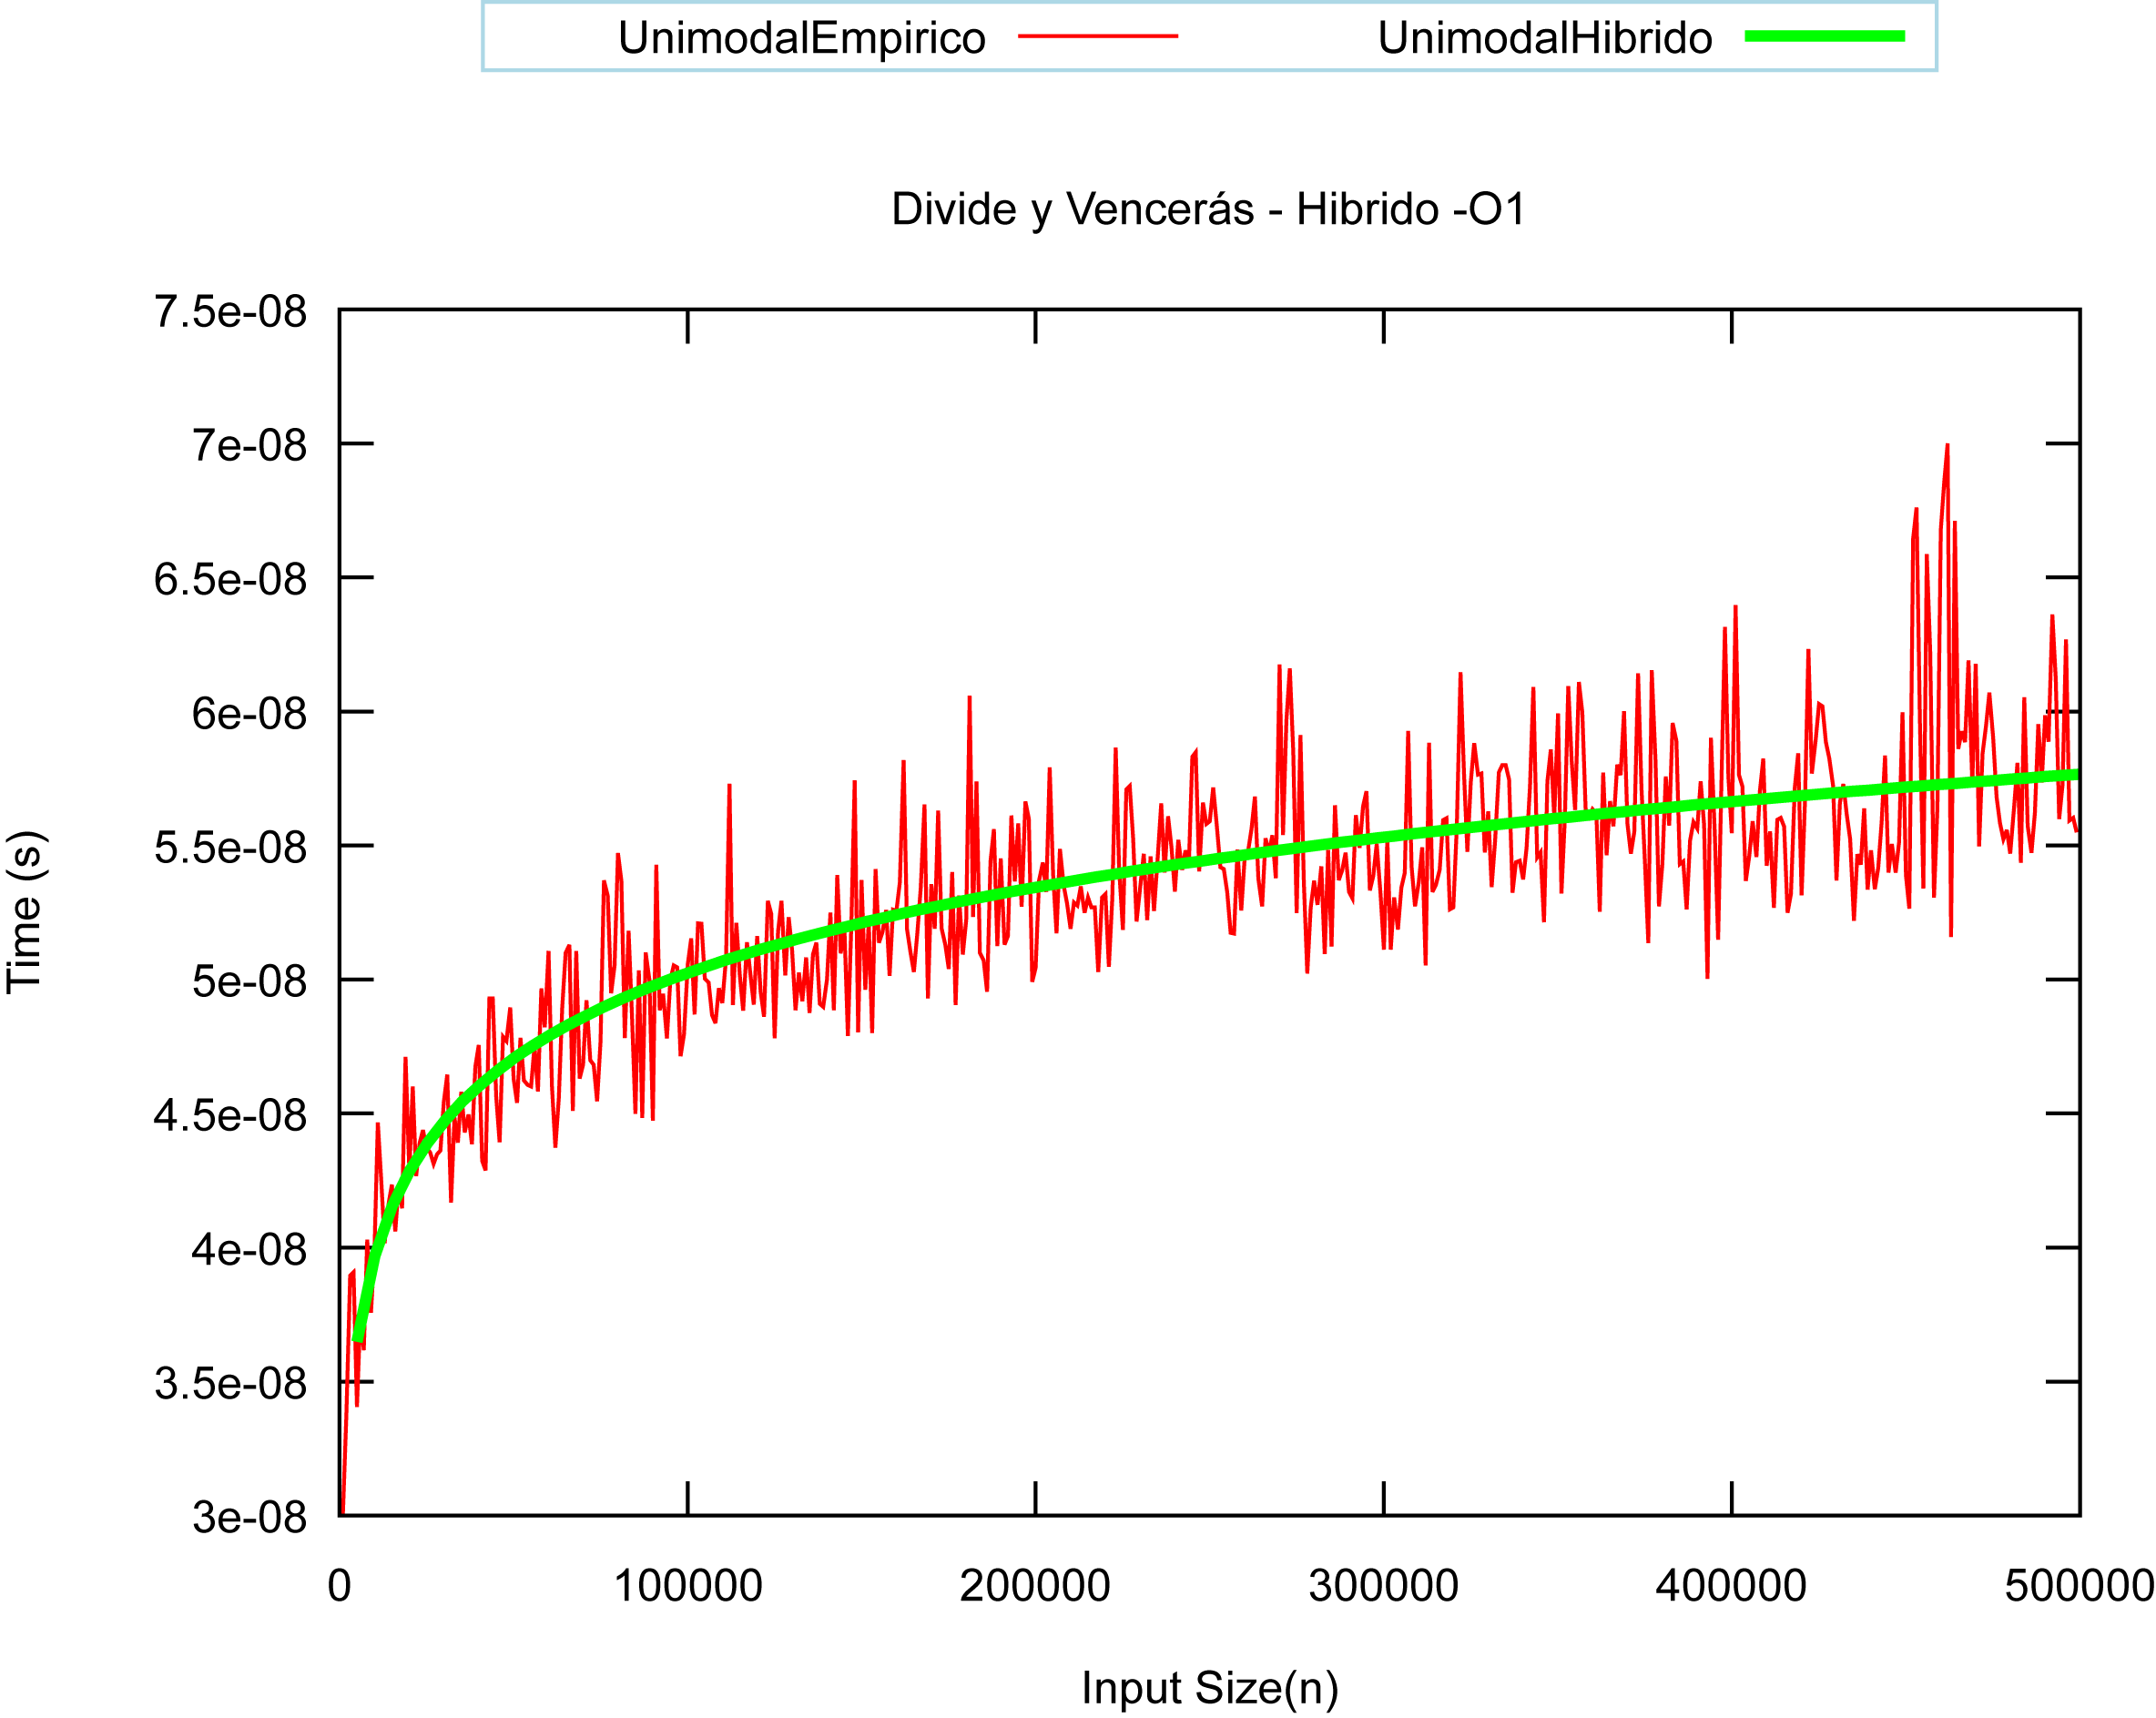
\includegraphics[width=8.6cm,height=7.1cm]{Images/dyv-hibridoO1}}
		\end{picture}
		\end{center}
		\end{figure}
		
\end{frame}	




\begin{frame}[plain]
	\frametitle{Constantes ocultas}
	
		\begin{defn}
			
			En este caso la función queda de la siguiente forma:
		
		\begin{equation}
			T(n) = 4.61006\cdot 10^{-09} \cdot log(n) - 2.83008\cdot 10^{-09}
		\end{equation}
	
		\vspace*{0.05in}
		
	\end{defn}
	
	

		
\end{frame}





\begin{frame}[plain]
	\frametitle{Optimización 2}
		\begin{figure}[htb]
		\begin{center}
		\begin{picture}(160,0)
		\put(-50,-110){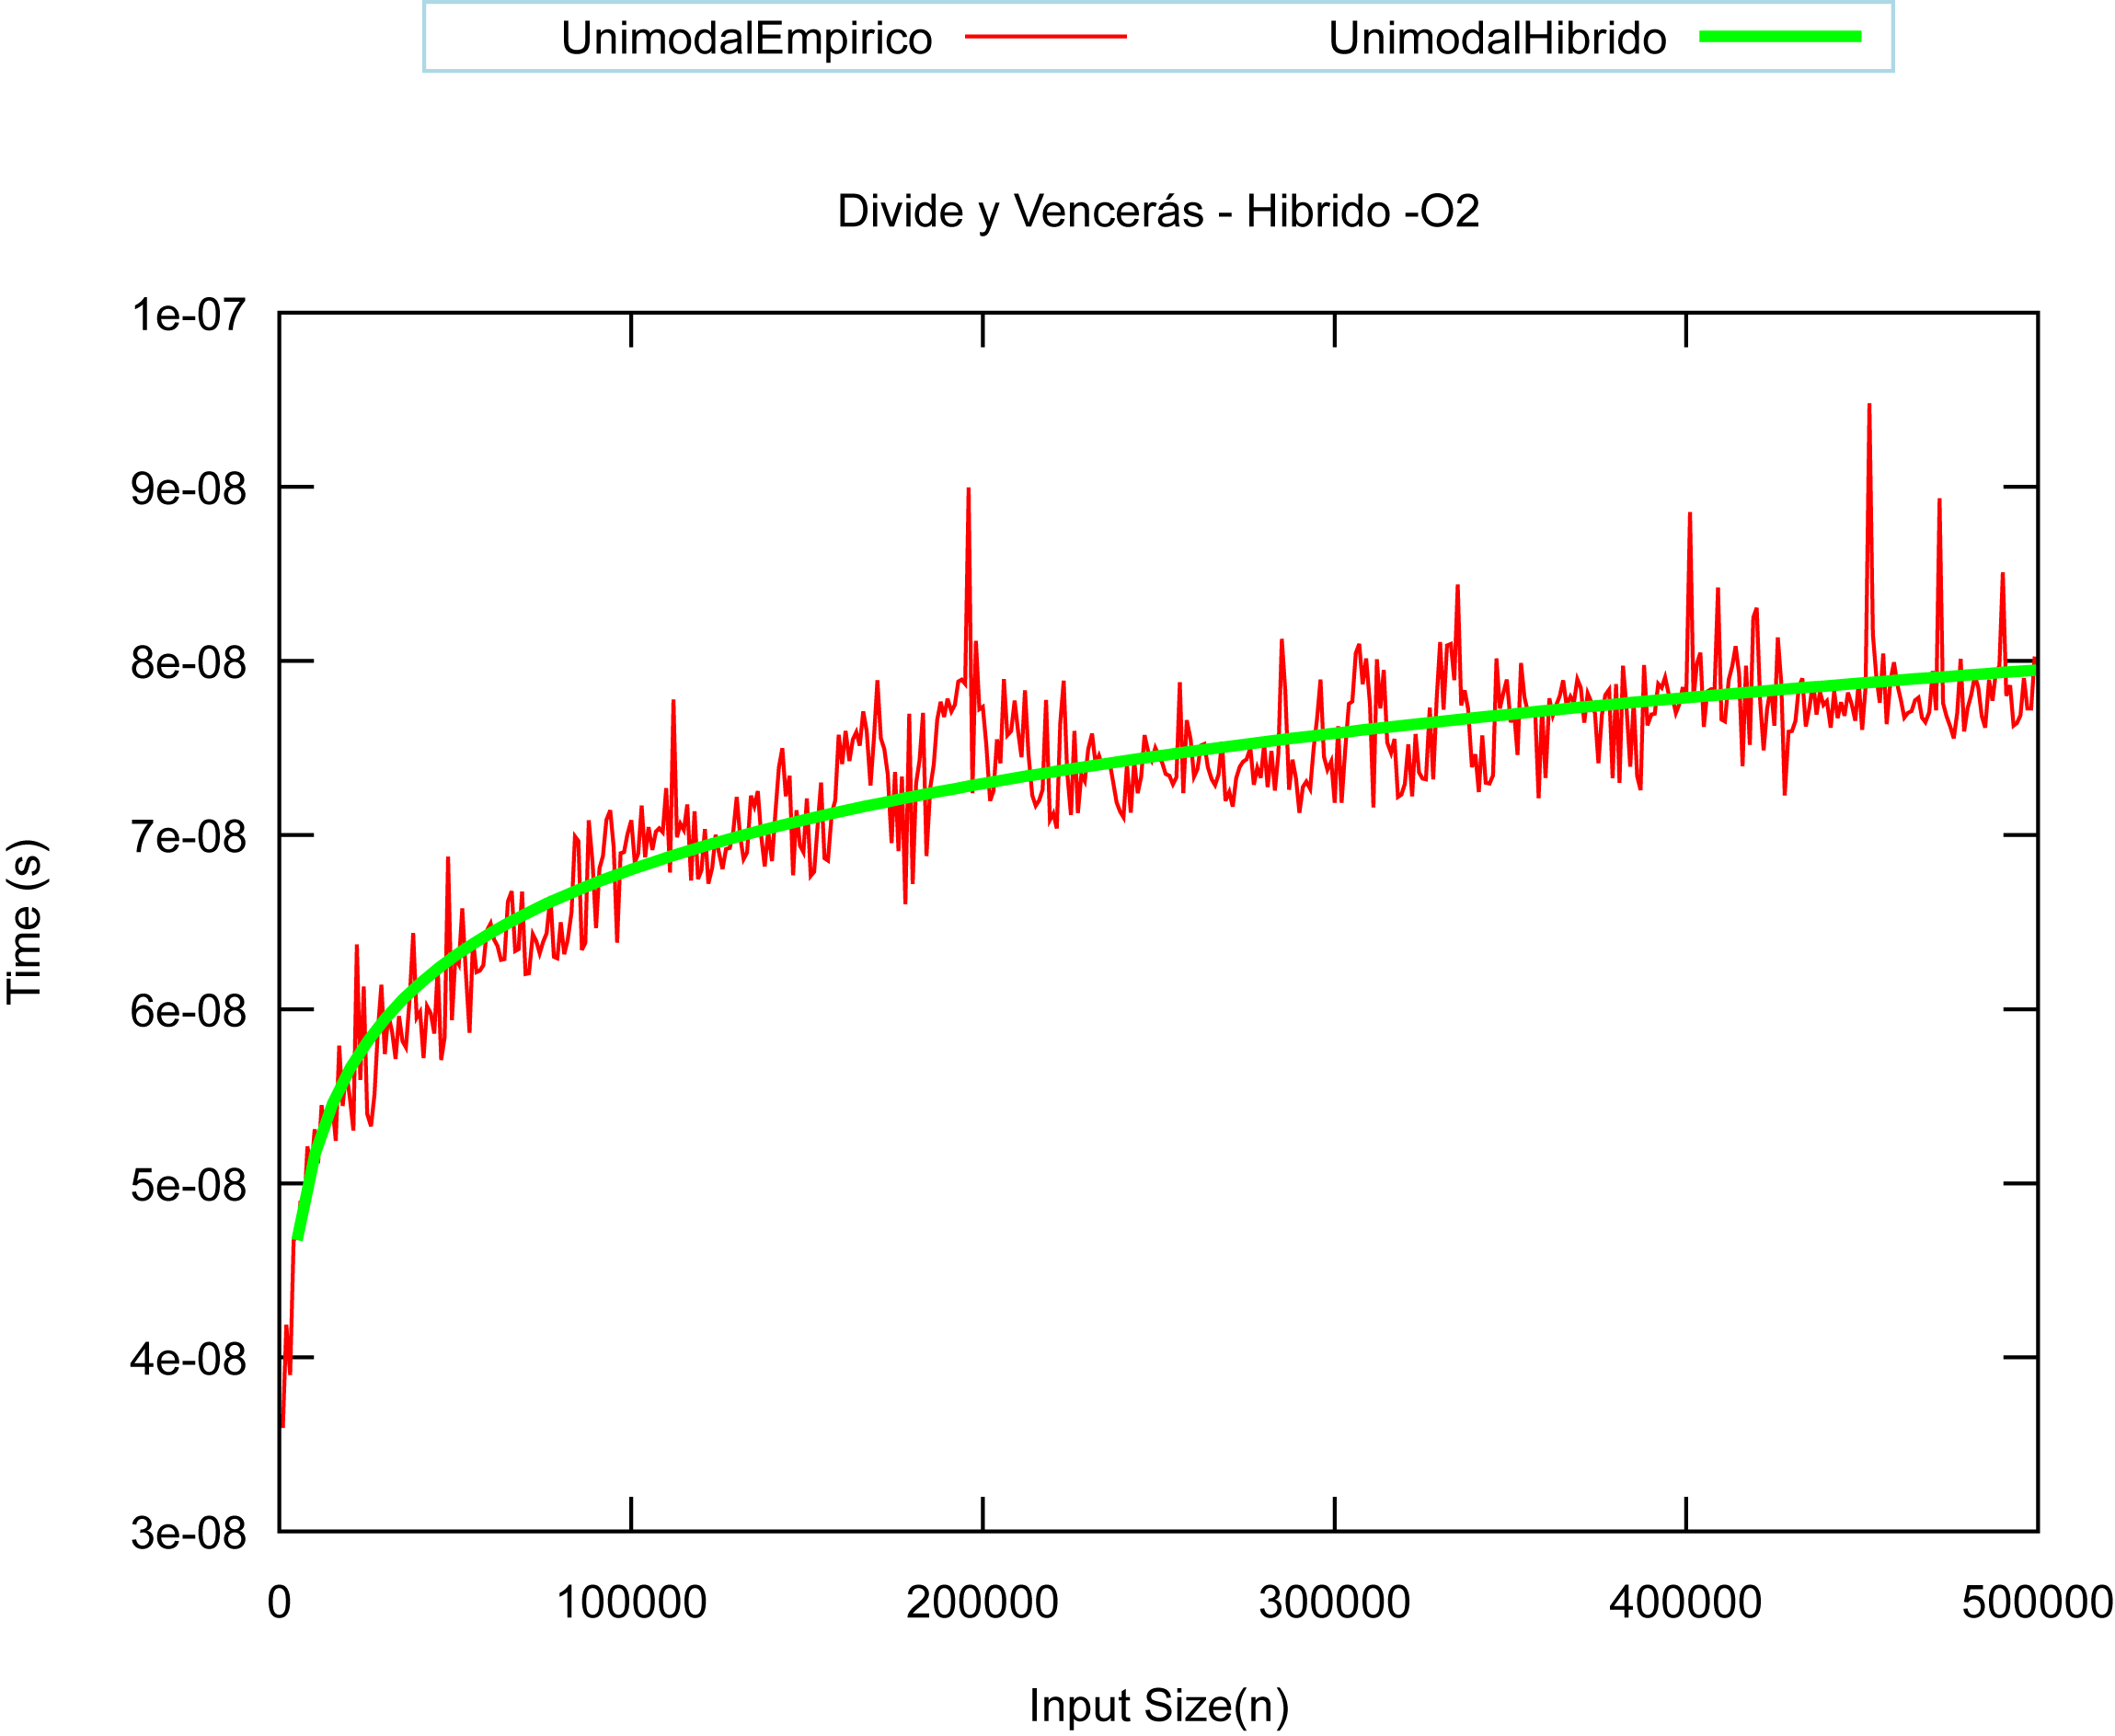
\includegraphics[width=8.6cm,height=7.1cm]{Images/dyv-hibridoO2}}
		\end{picture}
		\end{center}
		\end{figure}
		
\end{frame}	




\begin{frame}[plain]
	\frametitle{Constantes ocultas}
	
		\begin{defn}
			
			En este caso la función queda de la siguiente forma:
		
		\begin{equation}
			T(n) = 7.12567\cdot 10^{-09}  \cdot log(n) -1.4022\cdot 10^{-08} 
		\end{equation}
	
		\vspace*{0.05in}
		
	\end{defn}
	
	

		
\end{frame}







\begin{frame}[plain]
	\frametitle{Conclusión} 
	
	\begin{exampleblock}{Mejora}
			De nuevo, volvemos a ver que la mejoría se encuentra, como no podía ser de otra forma, en el valor de las constantes ocultas.
			También podemos observar que la mejoría es menos notoria si la comparamos con la mejora obtenida después de optimizar el algoritmo bruto hacia la optimización 1.
		\end{exampleblock}
\end{frame}		


		
		
		
	




	\section[Conclusiones]{Conclusiones}

	\begin{frame}[plain]
	\frametitle{Conclusión} 
	
	\begin{exampleblock}{Mejora}
		Hemos podido comprobar de primera mano que un cambio en en la optimización o en las prestaciones de la computadora donde se ejecute nuestro algoritmo hace variar las constantes multiplicativas. \\
		Estos cambios pueden ser sustanciales, pero un cambio de algoritmo puede variar la el orden de eficiencia, lo que nos lleva a un cambio mucho más drástico que el que nos proporcionan las constantes ocultas. \\
		Conclusión: mejorar el algoritmo es mejor que mejorar las prestaciones de nuestro ordenador.
	\end{exampleblock}

\end{frame}	
	
	\begin{frame}[plain]
	\frametitle{Tabla Optimizacion 0}
		\begin{figure}[htb]
		\begin{center}
		\begin{picture}(160,0)
		\put(-80,-100){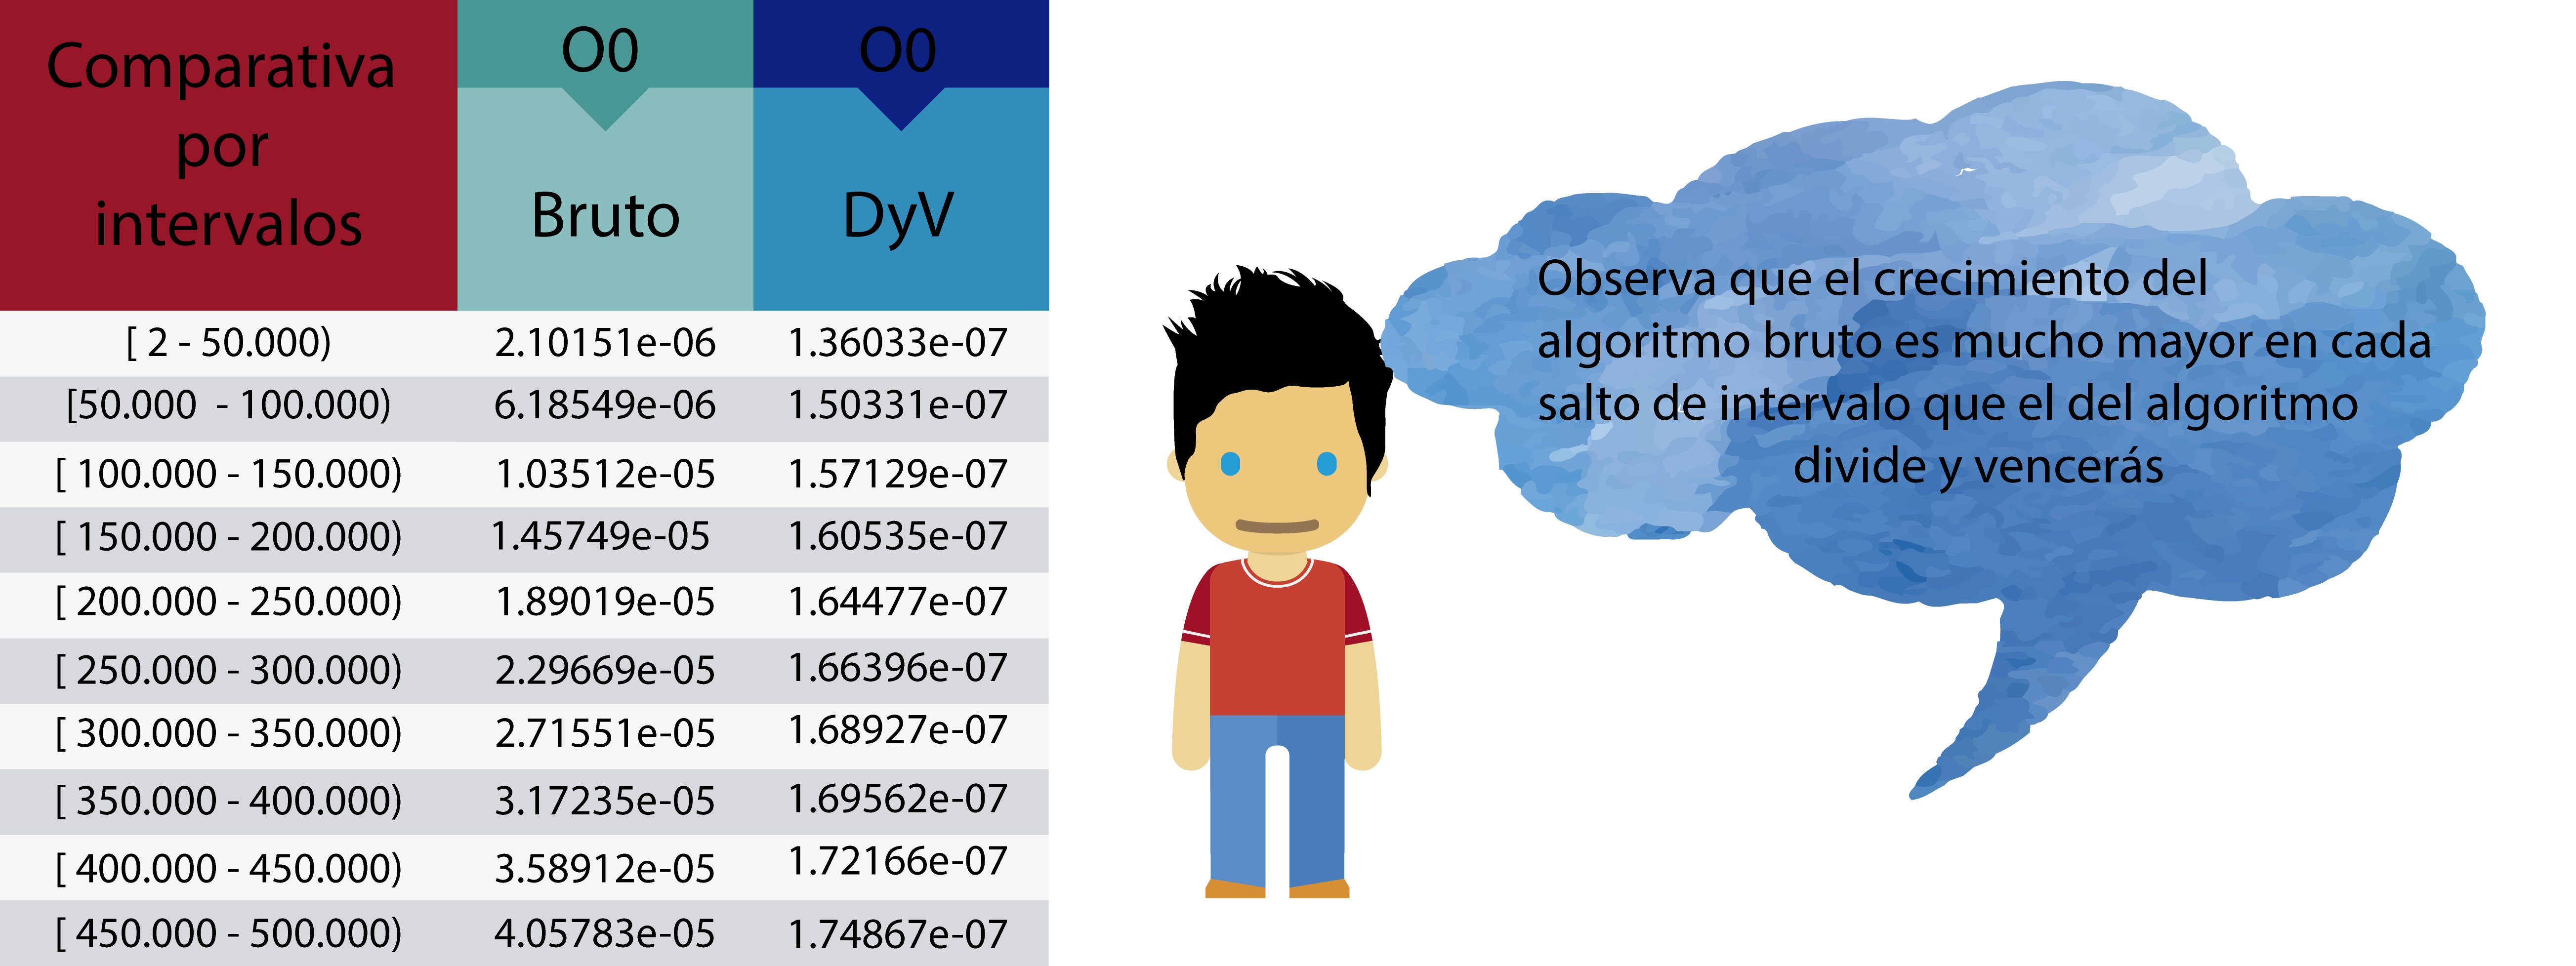
\includegraphics[width=12.0cm,height=5.3cm]{Images/TablaA-01}}
		\end{picture}
		\end{center}
		\end{figure}
		
	\end{frame}
	
	\begin{frame}[plain]
	\frametitle{Tabla Optimizacion 1}
		\begin{figure}[htb]
		\begin{center}
		\begin{picture}(160,0)
		\put(-80,-100){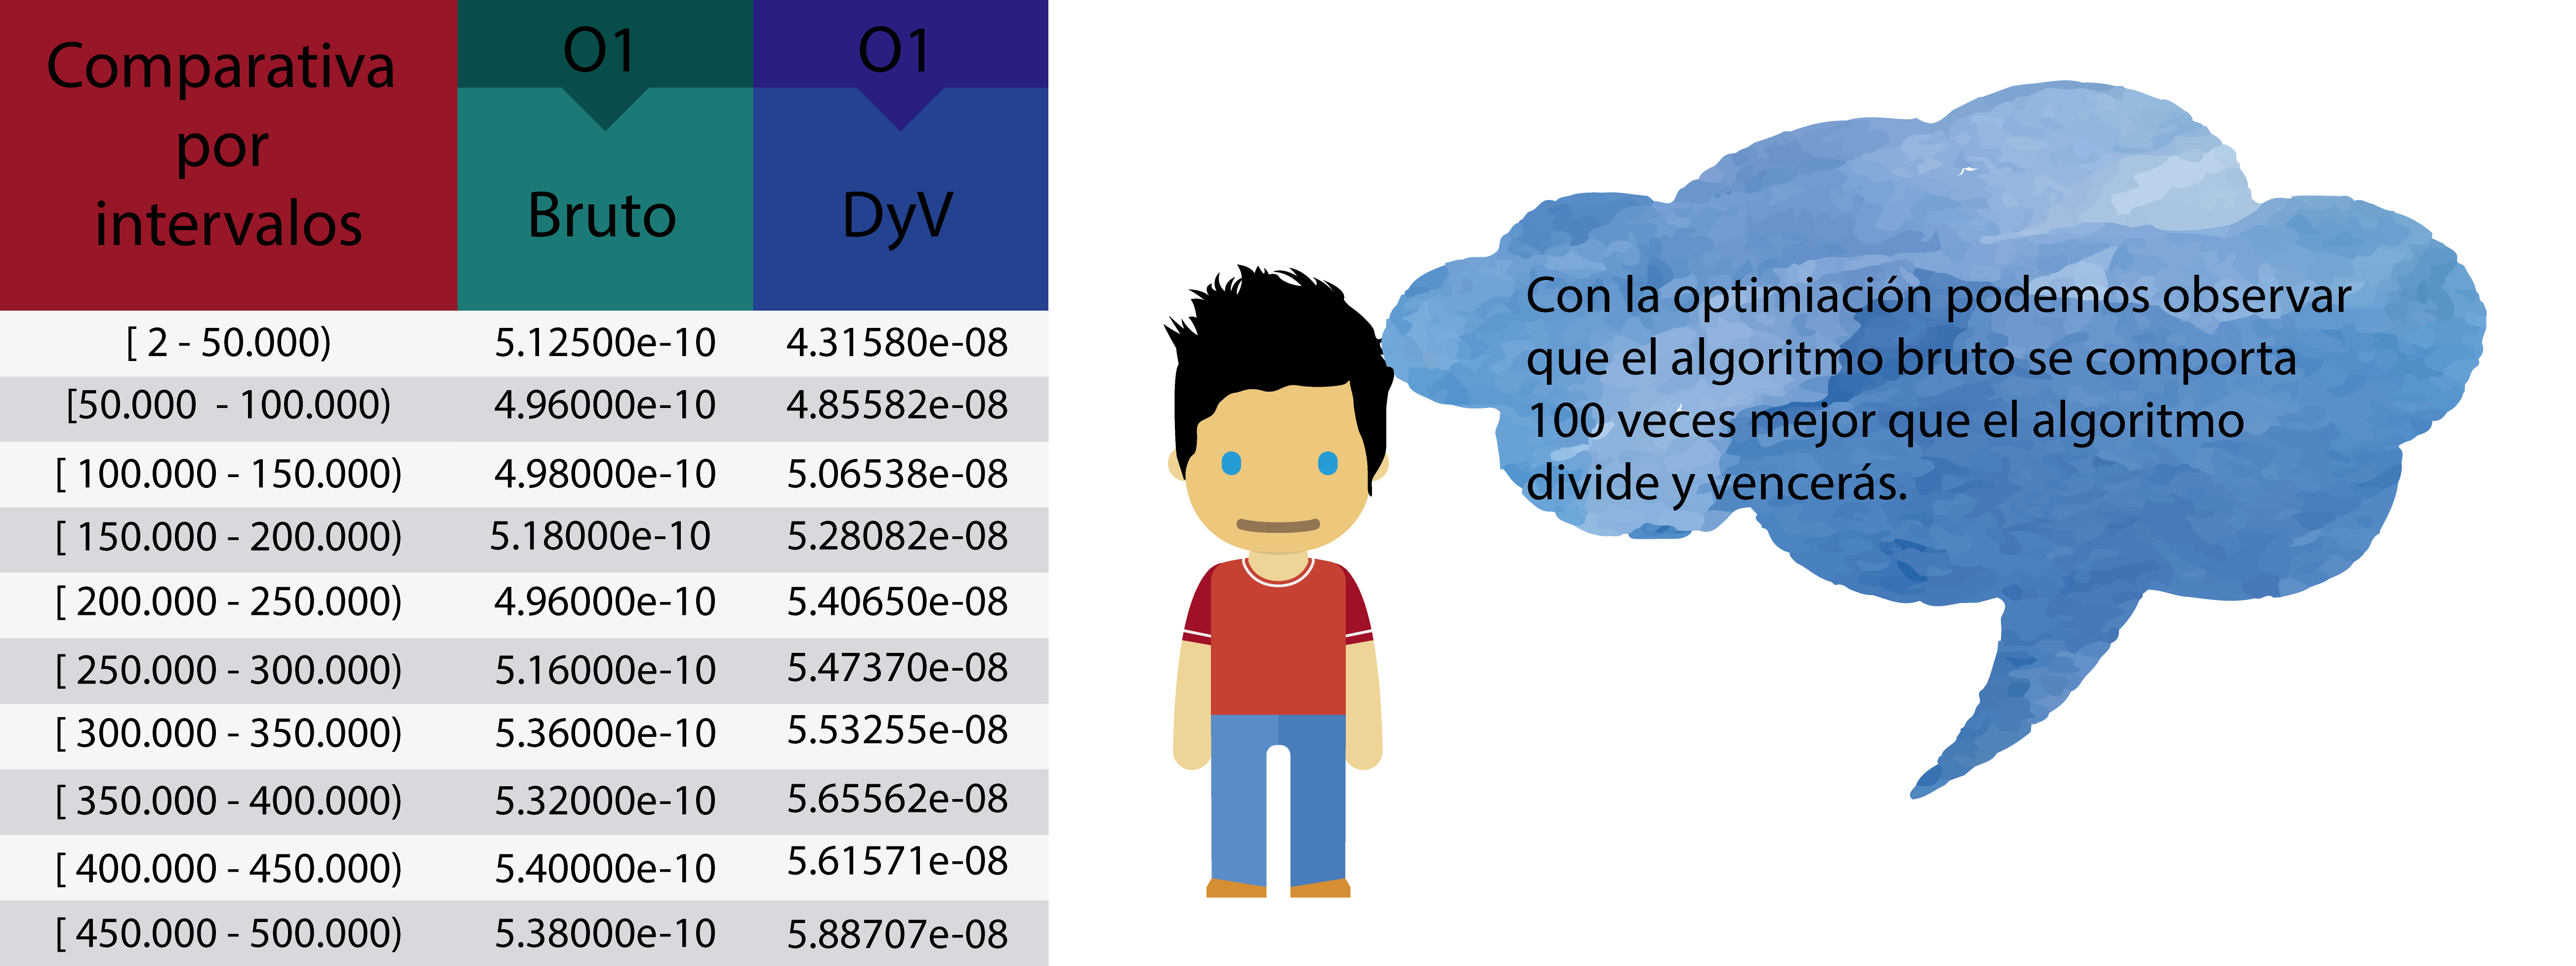
\includegraphics[width=12.0cm,height=5.3cm]{Images/TablaB-02}}
		\end{picture}
		\end{center}
		\end{figure}
		
	\end{frame}	
	
	
	
	\begin{frame}[plain]
	\frametitle{Tabla Optimizacion 2}
		\begin{figure}[htb]
		\begin{center}
		\begin{picture}(160,0)
		\put(-80,-100){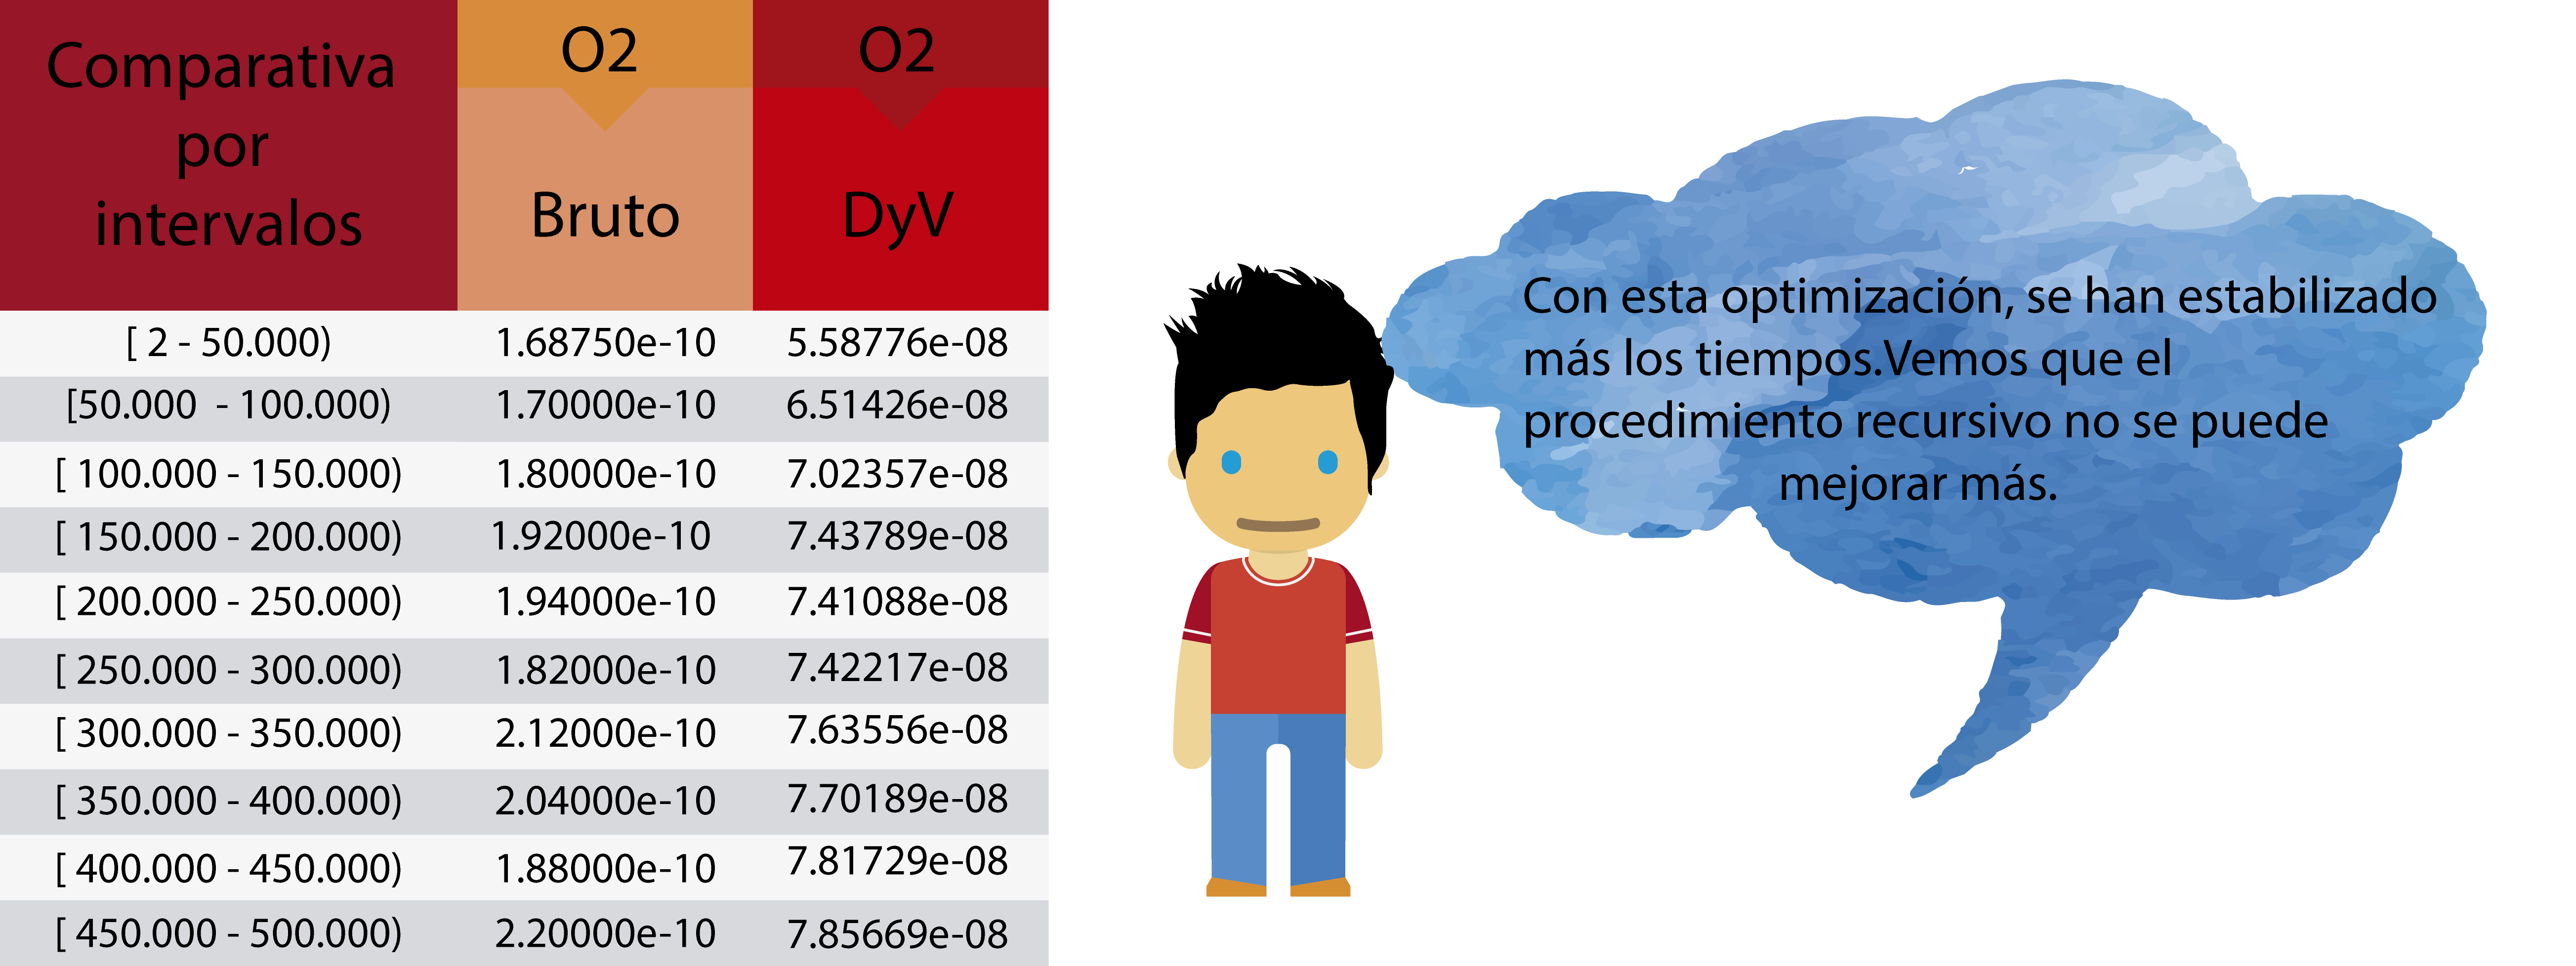
\includegraphics[width=12.0cm,height=5.3cm]{Images/TablaC-03}}
		\end{picture}
		\end{center}
		\end{figure}
		
	\end{frame}		


	\begin{frame}[plain]
	\frametitle{Tabla resumen}
		\begin{figure}[htb]
		\begin{center}
		\begin{picture}(160,0)
		\put(-95,-110){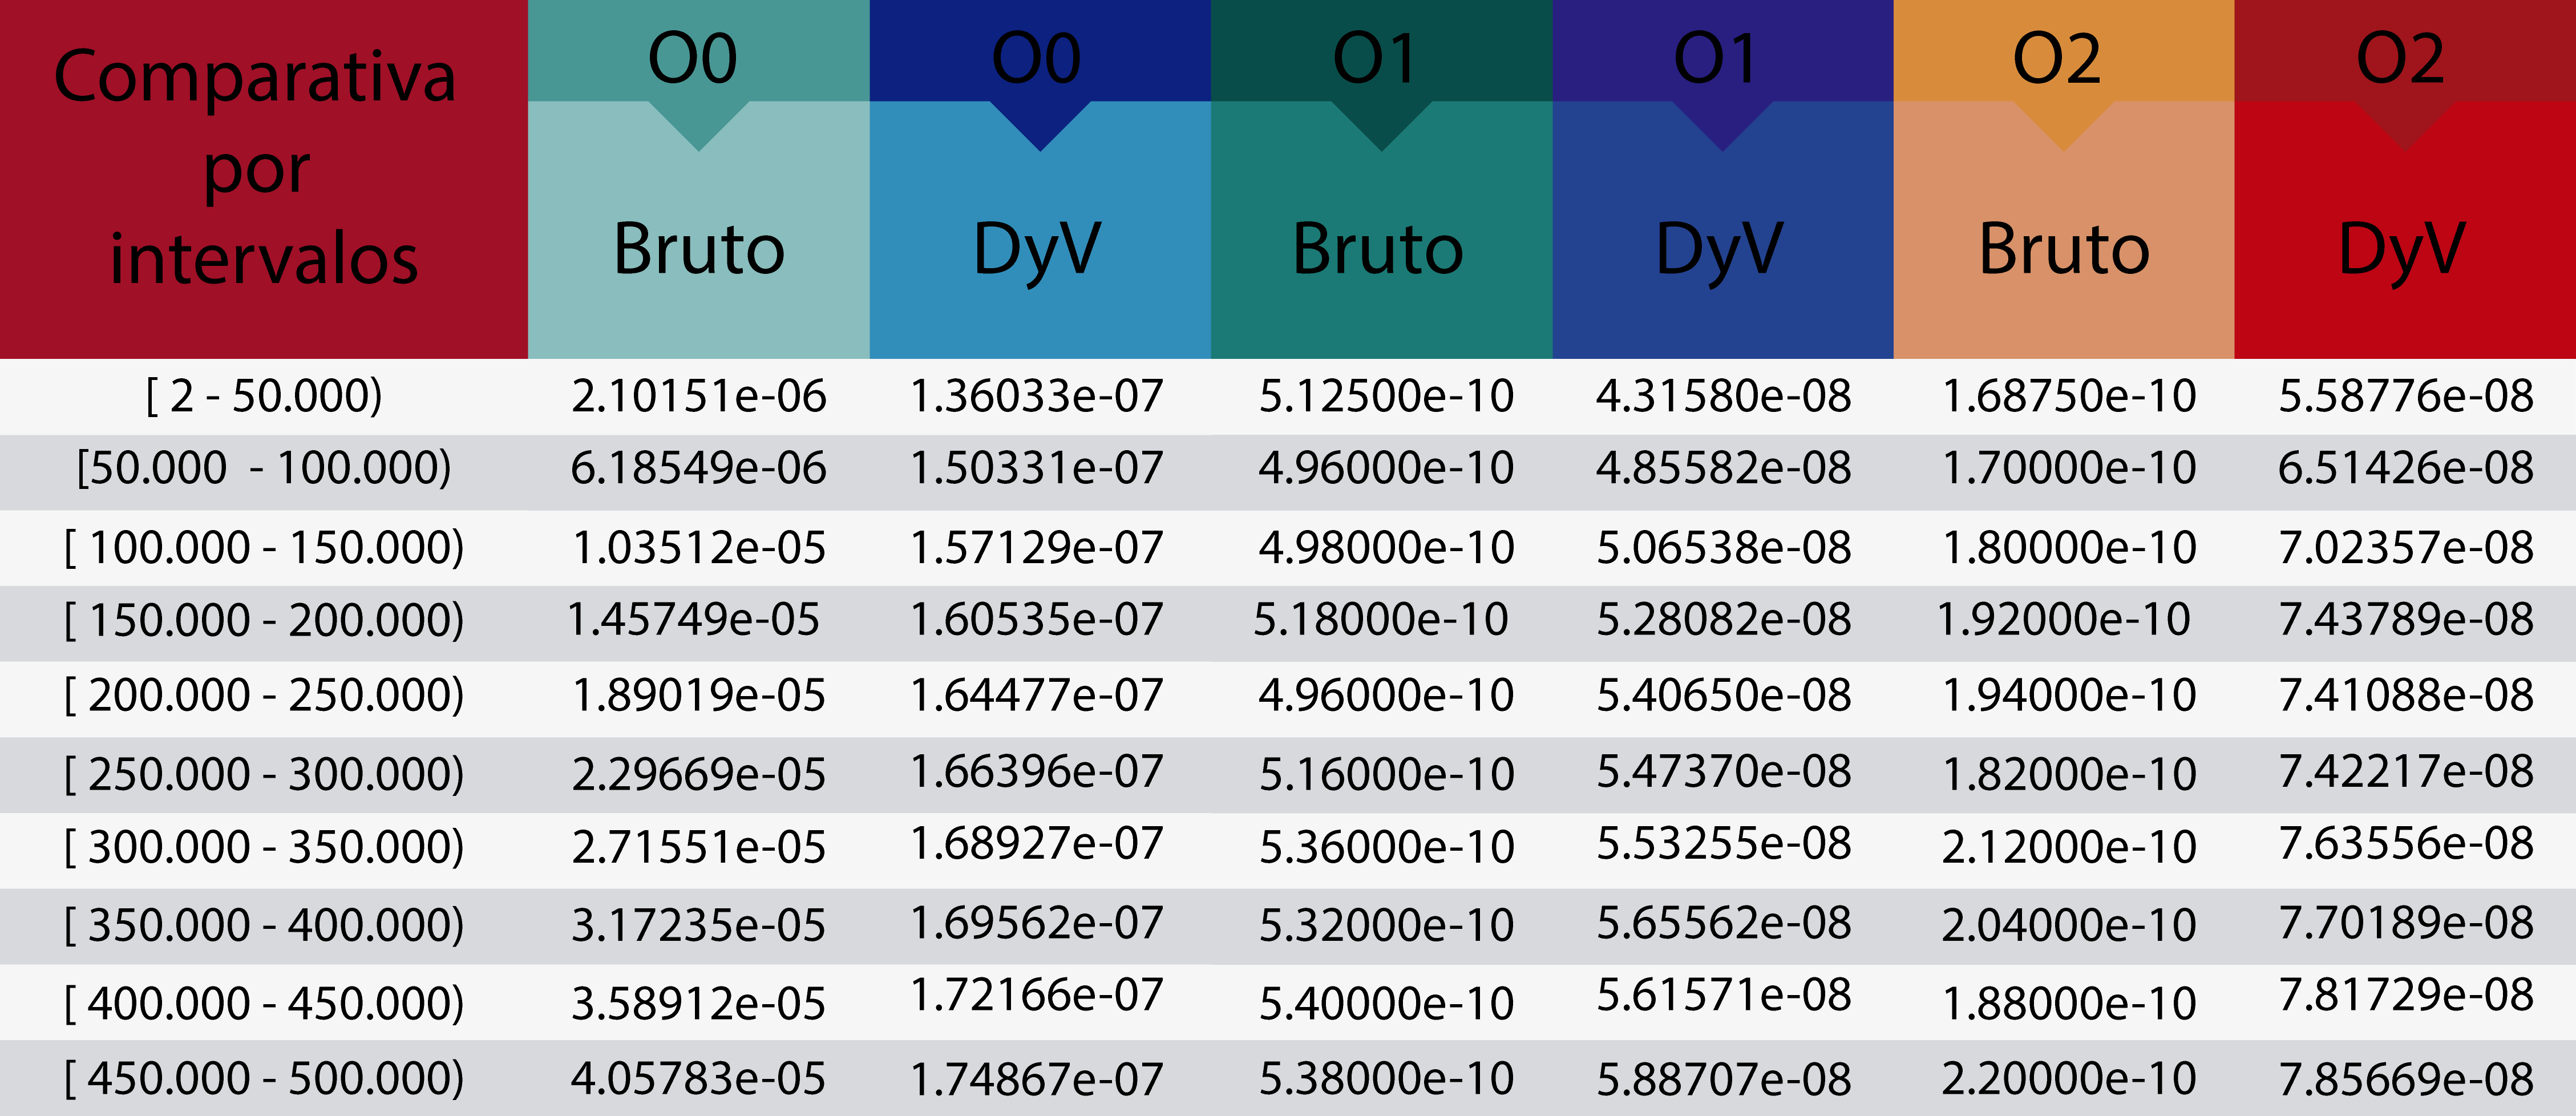
\includegraphics[width=12.1cm,height=6.9cm]{Images/TablaD-04}}
		\end{picture}
		\end{center}
		\end{figure}
		
	\end{frame}	
	
	\begin{frame}[plain]
	\frametitle{Agradecimientos}
		\begin{figure}[htb]
		\begin{center}
		\begin{picture}(160,0)
		\put(-110,-180){
\includegraphics[width=13.5cm,height=8.7cm]{Images/TablaAgradecimiento-05}}
		\end{picture}
		\end{center}
		\end{figure}
		
	\end{frame}	
	
	
	
	
	


	
	
	
	
	

	
	
	

\end{document}
